\documentclass[oneside]{article}
\usepackage{fullpage}
\usepackage[pdftex]{graphicx}
\DeclareGraphicsExtensions{.png,.pdf}
\graphicspath{{images/}}
\usepackage[dvipsnames,usenames]{color}
\usepackage{hyperref}
\usepackage{verbatim}
\usepackage[format=plain,font=small]{caption}
\usepackage[small]{titlesec}
\usepackage[round,sectionbib]{natbib}
\usepackage{amstext}
\usepackage{setspace}
\bibliographystyle{plainnat}
\renewcommand\rmdefault{bch}
\linespread{1.07} 

\newcommand\amin{\text{minor}}
\newcommand\amaj{\text{major}}

\setlength{\topmargin}{0.3in}
\setlength{\textheight}{7.5in}

\begin{document}
\doublespacing
\title{Glyph-maps for Visually Exploring Temporal Patterns in Climate Data and Models}
\author{Hadley Wickham$^1$, Heike Hofmann$^2$, Charlotte Wickham$^3$, Dianne Cook$^2$\\
$^1$Department of Statistics, Rice University\\
$^2$Department of Statistics, Iowa State University\\
$^3$Department of Statistics, Oregon State University}
\date{}

\maketitle

\begin{abstract}

The multivariate spatio-temporal nature of climate data makes it difficult to draw all of the aspects simultaneously. This paper describes the conceptualization and construction of a type of display, a glyph-map, that can show these multiple aspects. Glyph-maps are a specialization of multivariate glyph plots. Each spatial location is displayed with one glyph that represents the multiple measurements, often recorded over time, at that location. Glyph-maps allow the discovery of both local and global structure, with a particular focus on temporal relationships, important for studying climate change. They provide alternatives to colored, facetted maps, or statistical summaries such as principal components. Glyph-maps have been used sporadically for spatio-temporal data, and with the ideas and software described in this paper it will be easier to produce them. The conceptualization described here also will enable developing interactive versions of glyph-maps, and make it simpler to explore the perceptual effects of different scales. The methods are developed for rectangular gridded data, but with some clever processing, which is explained, it is possible to get good glyph-maps of irregularly gridded data. Guides and reference marks, for different types of glyphs used in the glyph-maps, are also discussed.

\end{abstract}

\section{Introduction}

Climate data are composed of multiple variables, such as temperature, ozone, precipitation, and winds, with a spatial and temporal context. The classic display for data of this type is a ``heatmap'', a tiled plot using color to display the value of the variable of interest at each location (see many examples in \citet{IPCC}, like Figure 2.11). When measurements are made at multiple time points it is reasonably common to display the data with small multiples~\citep{tufte:2001}, such as in Figure~\ref{fig:nasa-facet}. In this plot, a separate map is drawn for each month (columns) and year (rows), over a six year period of remotely sensed temperature data above Central America \citep{murrell:2010}. Color is used to display de-seasonalized temperature (residuals from a linear model containing year and month terms), where red is mapped to high values and blue to low. The most noticeable feature is the strong red patch in the equatorial Pacific beginning mid-1997 and tapering out during 1998. This is the El Ni\~no event, a major temperature anomaly (see for example, \citet{trenberth} or \url{http://www.esrl.noaa.gov/psd/enso/enso.description.html}.) More work is required to see more localized patterns, like cooler land temperatures seen in early years.


To read long-term or localized temporal patterns, this type of plot is cognitively challenging: the reader must play ``spot the difference'' from one small image to another. Large spatial structures such as El Ni\~no are clear but it is very difficult to extract the temporal pattern because it requires mentally differencing the images. Using a movie to render these small multiples can help, but small trends still fail to draw readers' attention and escape unnoticed \citep{simons:gradual}. The \emph{glyph-map} display described in this paper enables easier perception of temporal patterns. 

The glyph-map uses a small glyph, or icon, to represent multiple variables, or time values, at each location. Glyph-maps derive from glyph plots, which were initially developed to display multivariate data. One glyph is drawn for each observation in the data set. Types of glyph plots include the star plots \citep{mayr:1877, FD01, kleiner:1981}, the semi-graphic displays \citep{anderson:1960}, and the infamous Chernoff faces \citep{chernoff:1973}. A glyph is produced by mapping each variable to some graphical feature, such as the length of a line, curvature of the mouth, or size of the face. 

\begin{figure*}[htbp]
  \centering
  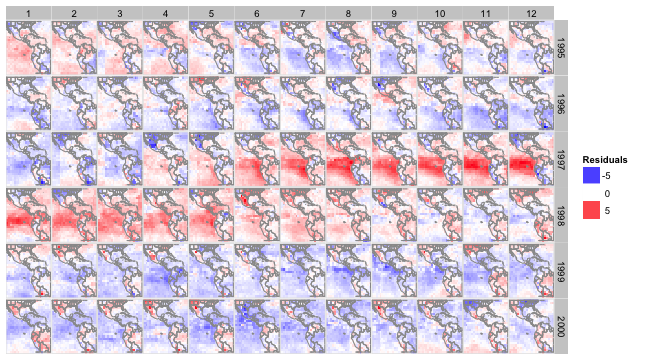
\includegraphics[width=5.5in]{nasa-colored-map.png}
  \caption{Facetted heatmap of de-seasonalized temperature. The dominant feature is the El Ni\~no warming in the southern equatorial region in the last half of 1997 and first half of 1998. Smaller features are only noticeable on closer inspection, or if pointed out: such as the relative warming on the mountain regions in South and North America which are red in all months in the later years.}
  \label{fig:nasa-facet}
\end{figure*}

\begin{figure*}[htbp]
  \centering
  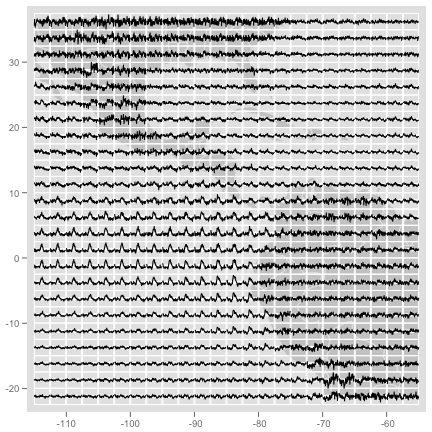
\includegraphics[width=3.5in]{nasa-deseas-glyph}
  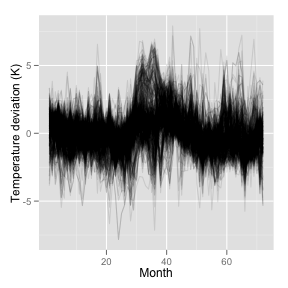
\includegraphics[width=2in]{nasa-deseas-glyph-leg}
  \caption{(Left) Glyph-map of de-seasonalized temperature, to compare with Figure \ref{fig:nasa-facet}. Time series of the six years of monthly temperature are plotted at each spatial grid location. The El Ni\~no appears as a bump in the middle of the time series, in the equatorial Pacific region. Large variations in temperature can be seen in areas over land, while being fairly constant over water. (Right) Glyph-map legend, showing temporal pattern without spatial pattern, giving the scale of the glyphs.}
  \label{fig:nasa-glyph}
\end{figure*}

Figure~\ref{fig:nasa-glyph} shows the glyph-map equivalent of Figure~\ref{fig:nasa-facet}: each location is represented by a small time series glyph of de-seasonalized temperature. The darker grey in the background represents the land mass of the study region. Because the data are de-seasonalized, the primary visible structure is still El Ni\~no, recognized by the bump in the middle of the series of the equatorial Pacific region. It is both a temporal anomaly and a spatial phenomenon, so this is not surprising. Other temporal features are visible from the many time series. Temperatures are generally more varied over land, than sea. A few locations, near the coast of South America and the southern part of North America, have dramatic jumps in temperature in the later years.

The glyph-map can also be thought of as a small multiple display~\citep{tufte:2001}. The primary comparison is different from the facetted heatmap. Cognitively, elements placed close to each other are more easily and accurately compared \citep{cleveland:1984}. The facetted heatmap, places greater emphasis on comparison between the spatial locations, because these are positioned together, and secondary emphasis on time because these are separated by facets. In the glyph-map, primary emphasis is placed on the temporal comparison, and secondarily on spatial comparison, because facetting is on spatial locations.  

In general, multivariate glyph displays lack a natural ordering because the observations have no ordering. Similarly, there are multiple ways that variables can be mapped to glyph properties, which can result in a combinatorial explosion of possible mappings, each producing a display that may emphasize some entirely different features of the data compared to another mapping. This may have prevented the widespread adoption of glyph displays, despite some proposed ordering solutions \citep{kleiner:1981,hurley:2010}. Using glyphs with space-time data eliminates the ordering issue: glyphs are placed according to the location of the measurement, and variables are ordered by the time they were collected. Additionally, climate data usually has high correlations between nearby locations and times, imposing a degree of smoothness that gives the plot an appearance of a textured  landscape, which makes it easier to digest patterns from one glyph to another. Others \citep{pickett:1988} have used glyphs on maps to display multivariate spatial data. This area of work has morphed into the field of metaphorical data displays, which create abstract landscapes of spatial data, a digression from glyph-maps. \citet{gribov:2006} describes the use of glyph-maps for multivariate data also, with emphasis on the graphics software, Gauguin. Glyph-maps for spatiotemporal data have been used in several publications \citep{carr:1992,eden:2010,hobbs:2010}. Glyph-maps using arrow glyphs have commonly been used for displaying ocean currents, wind direction and strength, as can be seen in the Figure 8.1  and a rudimentary time series glyph display can be seen in Figure 9.12 of \citet{IPCC}. 

Another common approach for displaying spatiotemporal data is to calculate a statistical summary for each location and display these values as single heatmap. For example, to study long-term trends, the slope of a linear model can be calculated at each location and color tiles used to display the slope value over space. This approach is less than exploratory, in the sense that it requires a pre-conceived definition of the relationship of interest, and clean data so that the summary statistic adequately summarizes the pattern. 

Two types of glyph -- lines and stars -- are especially useful for temporal displays. Figure~\ref{fig:templates} plots 12 iconic time series shapes (linear increasing, decreasing, shifted, single peak, single dip, combined linear and nonlinear, seasonal trends with different scales, and a combined linear and seasonal trend) as line- and star-glyphs. The data underlying each glyph is measured at 36 time points. The line-glyphs are   time series plots. The star-glyphs are formed by considering the 36 axes radiating from a common midpoint, and the data values for the row are plotted on each axis relative to the locations of the minimum and maximum of the variable. This is a polar transformation of the line-glyph.

\begin{figure}[htbp]
  \centering
  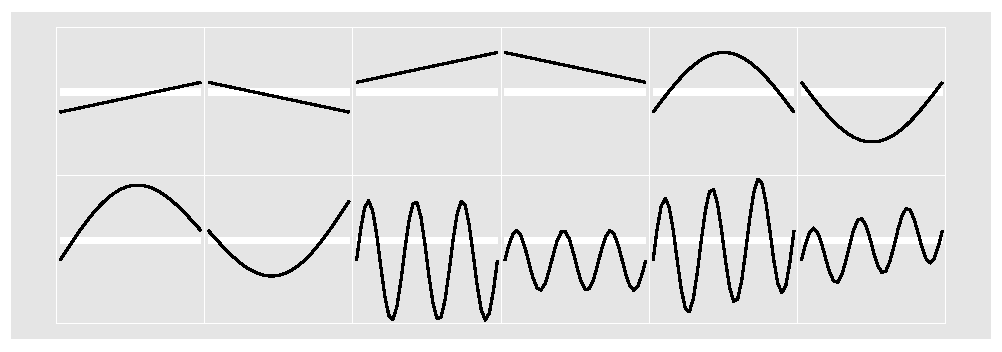
\includegraphics[width=0.5\linewidth]{euclid-to-polar-1}%
  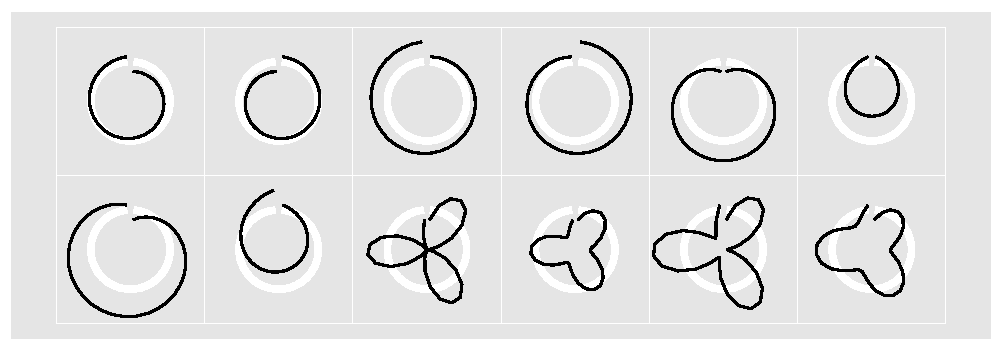
\includegraphics[width=0.5\linewidth]{euclid-to-polar-2}

  \caption{Icon plots for 12 iconic time series shapes (linear increasing, decreasing, shifted, single peak, single dip, combined linear and nonlinear, seasonal trends with different scales, and a combined linear and seasonal trend) in Cartesian coordinates, time series icons (left) and polar coordinates, star plots (right). White reference grids, lines and circles are added to help compare the shapes.}
  \label{fig:templates}
\end{figure}

Section~\ref{sec:construction} describes the algorithm used to create glyph-maps of these two types of glyphs. Section~\ref{sec:perception} discusses their perceptual properties, including the importance of visual reference grids, and of careful consideration of scale. Large data and the interplay with models and data are discussed in Section~\ref{sec:large-data}. Many spatiotemporal data sets have irregular spatial locations, and Section~\ref{sec:irregular} discusses how glyph-maps can be constructed for this type of data. Three datasets are used for examples:

\begin{quote}
\begin{itemize} \itemsep 0in

\item[EXPO] The ASA 2009 expo data \citep{murrell:2010} consists
  of monthly observations of several atmospheric variables from the
  International Satellite Cloud Climatology Project. The data set
  includes observations over 72 months (1995--2000) on a 24 x 24 grid
  (576 locations) stretching from $113.75^{\circ}$W to
  $56.25^{\circ}$W longitude and $21.25^{\circ}$S to $36.25{^\circ}$N
  latitude.

\item[GISTEMP] Surface temperature data provided on $2^{\circ}$ x
  $2^{\circ}$ grid over the entire globe, measured monthly
  \citep{GISTEMP} from 1880-2011. To produce this data irregularly
  gridded ground station data was de-seasonalized, differenced from
  the 1951-1980 temperature averages, and spatially averaged to obtain
  gridded temperature anomalies. For the purposes of this paper, we
  extracted the locations corresponding only to the continental USA.

\item[USHCN] (Version 2) Ground station network of historical
  temperatures \citep{USHCN}. Temperatures from 1219 stations on the
  contiguous United States, from 1871 to present.
  
\end{itemize}
\end{quote}
Supplementary material contains the data sets and code to reproduce the plots in this paper.  R \citep{R} with the packages {\tt ggplot2} \citep{me:ggplot2} and {\tt plyr} \citep{me:plyr} was used. 

\section{Structural components}~\label{sec:construction}

It is useful to recognize that the glyph-map is a linear mix of two structural components of the data: spatial location and data values. The spatial location is the major positioning component, while the data values are minor adjustments to those positions. For spatiotemporal data, the major components are longitude ($s_x$) and latitude ($s_y$), and the minor components are time ($t$) and some variable ($z$), for example, temperature, or predicted temperature. Assuming the minor components ($t, z$) are scaled into the range $[-1, 1]$, the final coordinates $(x,y)$ of the values in the plot are the linear combination, given by:

\begin{equation}
  \begin{array}{lll}
  x &=& s_x + \alpha_x \cdot w \cdot t\\
  y &=& s_y + \alpha_y \cdot h \cdot z, 
  \end{array}
  \label{coords.eqn}
\end{equation}

\noindent where $\alpha_x, \alpha_y$ are scale parameters setting the fraction of width, $w$, and height, $h$, of the glyph, respectively. For gridded data, $w$ and $h$ will be the minimum difference between neighboring spatial locations to make use of the resolution of the major components. For irregularly gridded data, $w$ and $h$ would be set to minimize overlap between glyphs.

This way of thinking of the glyph-map is convenient for several reasons. The first is, that it moves the plots beyond the small multiples, many little plots, approach. That provides flexibility to cover large spatial domains using potentially tiny glyphs. A second, and major, reason is that with this approach they can then readily be made interactive. Different variables can be swept into, and out of, the minor axes using mouse motion that maps to $\alpha_x, \alpha_y$. Interactive glyph-maps were used to explore the EXPO data using  GGobi \citep{swayne:2003}, and then later reproduced in publication quality resolution using {\tt ggplot2} \citep{me:ggplot2} in \citet{hobbs:2010}. In GGobi, a manual tour is used to make the linear combination of spatial variables with other variables \citep{CB95}, and Equation \ref{coords.eqn} makes this approach more explicit, and generalizable beyond tours. The third reason is that it enables adjusting scales of glyphs in multiple ways to vary the emphasis, which is discussed in Section \ref{sec:perception}.

Coordinates for star glyphs are computed with a polar transformation of the minor components $(t, z)$:  

\begin{equation}
  \begin{array}{lll}
  x &=& s_x + \alpha_x \cdot z \cdot w \cdot \sin(2 \pi t) \\
  y &=& s_y + \alpha_y \cdot z \cdot h \cdot \cos(2 \pi t).
  \end{array}
  \label{coords.polar.eqn}
\end{equation}

\noindent where $(t, z)$ have been scaled into the range $[0, 1]$. This is a non-standard conversion to polar coordinates, but it creates a timeline that starts at 12 o'clock and proceeds clockwise. \citet{eden:2010} wrap the time series, overplotting the multiple years, and this could be done also, by adjusting the scale of $t$. 

Figure~\ref{fig:templates} gives some iconic examples of time series, shown both in Cartesian coordinates and polar coordinates. Differences between linear and nonlinear trend are more apparent in the line-glyphs, and are effectively lost in the star-glyphs, which are most effective in exposing cyclical patterns due to seasonality. Star-glyphs show seasonality as floral cartoons, with peaks forming petals. Opposing linear trends (up vs down) in line-glyphs are not readily seen in the star-glyphs, appearing only as differences in the gaps at the top of each glyph. The internal area of the star-glyphs reflects to the average value of a time series, while its shape shows deviations from the average.

\section{Perception}~\label{sec:perception}

All plots facilitate some comparisons and impede others. For a plot to be useful for a particular data analytic task, the display needs to make the primary comparisons the simplest to make. For climate data, changes in slope, or trend, average value, and variance over time, are the primary tasks. Glyph-maps support these tasks because the pieces of the graphical elements that are needed to make the temporal comparisons are organized, and grouped together.

Glyph-maps allow time trends to be read directly from the plot. Values are mapped to position, one of the easiest properties to perceive, rather than color, which is among the hardest graphical element to parse \citep{cleveland:1984}. Perceiving time trends in faceted heatmaps is much more difficult: not only do you need to read value from color (difficult), you also need to spot the difference (major challenge) between the different maps. From a cognitive perspective these sorts of comparisons can suffer from \emph{change blindness}, often leading to failure to notice the change and not knowing that something changed \citep{healey:2011,busey}. To see this, examine Figures~\ref{fig:nasa-facet} and \ref{fig:nasa-glyph}. The heatmap requires comparing color values across maps to assess temporal change but the glyph-map allows direct reading of the temporal trend at each location, and comparison across spatial neighbors. Conversely, if the purpose is to read spatial trend for one time point the heatmap may be a better choice, because this is a difficult task with the glyph-map. 

A possible draw-back of the glyph-map, particularly if linear trend is displayed as an icon, is it may suffer from the Z\"ollner Illusion \citep{Zollner}, which makes straight lines look crooked (Section \ref{sec:large-data} has an example).

Two other factors are critical for accurate perception of change: reference frames and scaling. These are described in the following two sections.

\subsection{Reference frames}~\label{sec:reference}

The structured spatial arrangement of icons in a glyph-map helps to compare the patterns of shape, like slope, intercept, or size, across icons. However, additional clues can make comparisons easier, converting the perceptual task from comparing length to the easier task of position along a common scale \citep{cleveland:1984}. This is also called a \emph{visual reference grid} \citep{cleveland:1993a}.

Each glyph is small, so there is not enough space for a full set of axes on each, and it is not desirable beause it would be repetitive, redundant information. Instead, minimal reference lines and boxes are incorporated. These need to be minimally perceptible, post-attentive \citep{healey} and de-emphasized, so as not to detract from the data. The reference grid is a box, framing each icon, which represents the spatial grid. The reference line is a horizontal line at mid-range. Both help to read differences in slope and intercept. Slope is read by comparing the position of left and right endpoints on the frame, or by reading the angle between the data line and the reference line. Intercept is read from ``average'' position of the line in the box: is it near the top, or near the bottom? Figure~\ref{fig:ref-basic} demonstrates both guides. Reference elements are drawn in white, so they are minimally perceptible relative to the black data elements. Average temperatures were calculated for each month, and these were passed to the glyph calculations to produce the glyph-maps.   For star glyphs the reference frames are also useful and the equivalent of the reference line is a circle (see Figure~\ref{fig:templates}).

\begin{figure}[htbp]
  \centering
  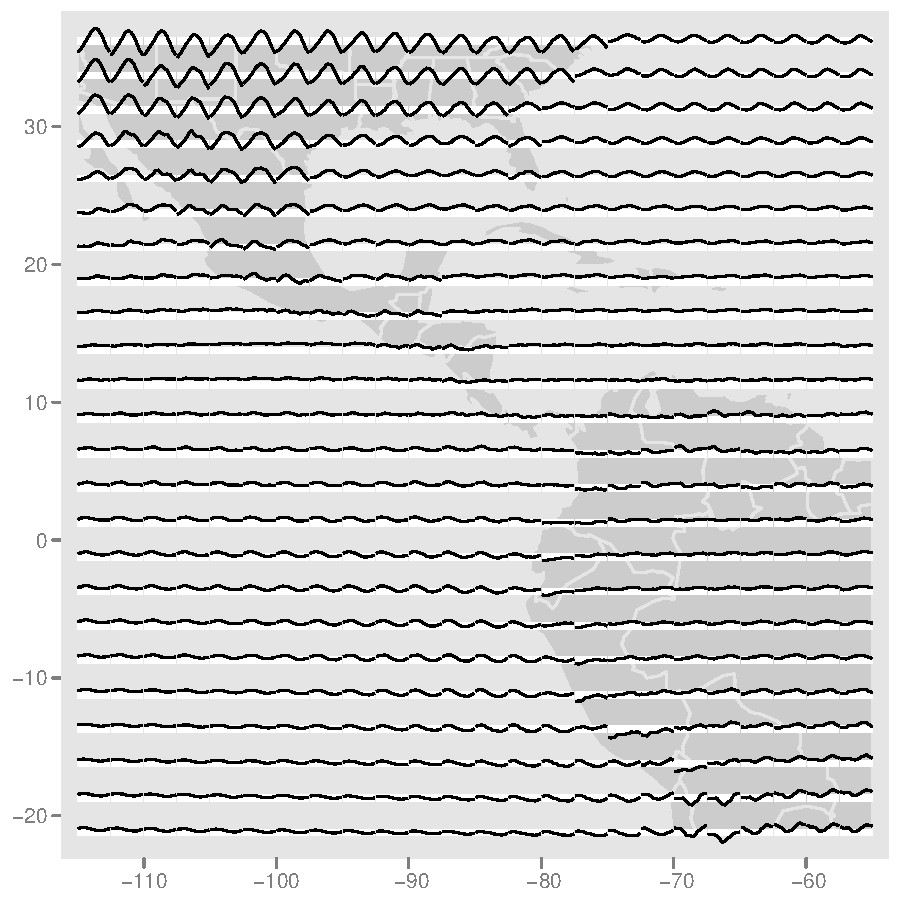
\includegraphics[width=0.5\linewidth]{ref-line}%
  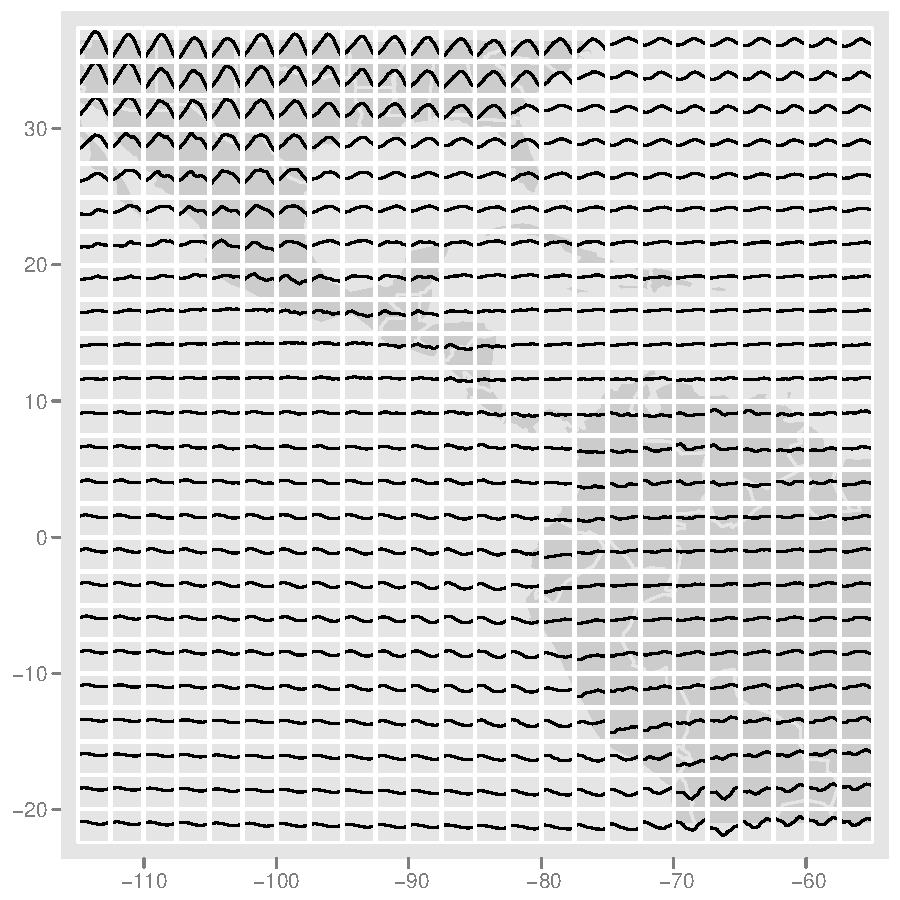
\includegraphics[width=0.5\linewidth]{ref-box}

  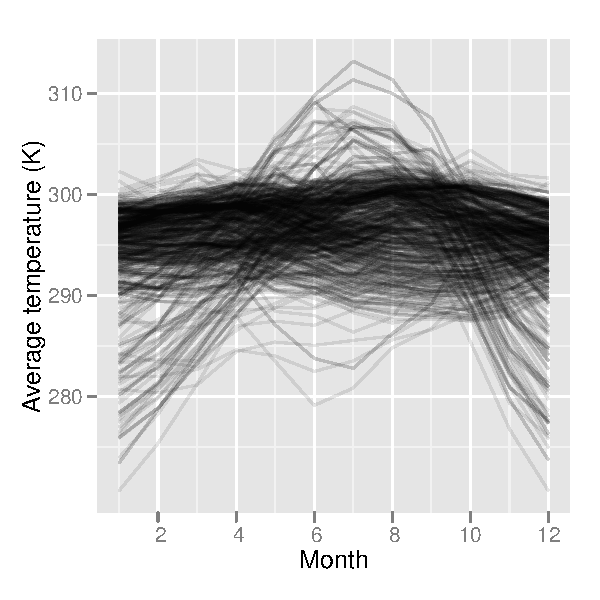
\includegraphics[width=0.33\linewidth]{ref-legend}

  \caption{Glyph-maps of seasonal temperature patterns (averages for each month over all years), using the EXPO data. Adding mid-range reference lines (top left) and grid-cell reference boxes (top right), makes it easier to see differences in glyph position, not just shape. (Bottom) Legend shows temperature values across all locations to aid interpretation.}
  \label{fig:ref-basic}
\end{figure}

To observe the scale of the measurements represented by the glyphs secondary legend plot is generated and displayed alongside the glyph-map, of all the glyphs overplotted, with complete axes. See, for example, Figure \ref{fig:nasa-glyph} where from the legend it can be seen that months range from 0 to 72 and de-seasonalized temperature ranges from -8 to 8$^0$K. In Figure \ref{fig:ref-basic}, months range from 1 to 12, and temperature from 270 to 315$^o$K.

\subsection{Scaling}~\label{sec:scale}

Different features of the data can be emphasized by varying the scale of $t, z$ (Equation \ref{coords.eqn}, \ref{coords.polar.eqn}) used within each cell. By default, a global scale, using the overall minimum and maximum of all $t, z$ values, is used to scale the measurements into the range $[-1, 1]$ (or $[0, 1]$ for polar coordinates). Then the range of values in one cell is comparable to those in other cells -- the same position within each cell corresponds to the same value in all locations. This facilitates the comparison of absolute values, and draws attention to locations with large overall variation. Alternatively, local scale can be used. With local scaling, the minimum and maximum values of $t, z$ are calculated for each location, and these are used to scale $t, z$ into the range $[-1, 1]$ (or $[0, 1]$). This makes it easier to compare shape (ignoring amplitude), and draws attention to locations with large relative variation. 

Figure~\ref{fig:scaling} compares global scaling and local scaling for the smoothed temperature data from the EXPO data. (The model is more complicated than the model used previously to de-seasonalize the data. A generalized additive model \citep{wood:2006} with qualitative month and smoothed day terms was fit to the observed data and predicted values were computed for each day of the six year period. Seasonal effects are removed but not overall average or long-term trend.) On the global scale, the El Ni\~no blip in temperature is just visible, along with variation in the average temperature at each location. Local scaling emphasizes the individual shapes: the impact of El Ni\~no can be seen to be over a wider region, along with linear increases in parts of South America, and decreases in the Gulf of Mexico.

\begin{figure}[htbp]
  \centering
  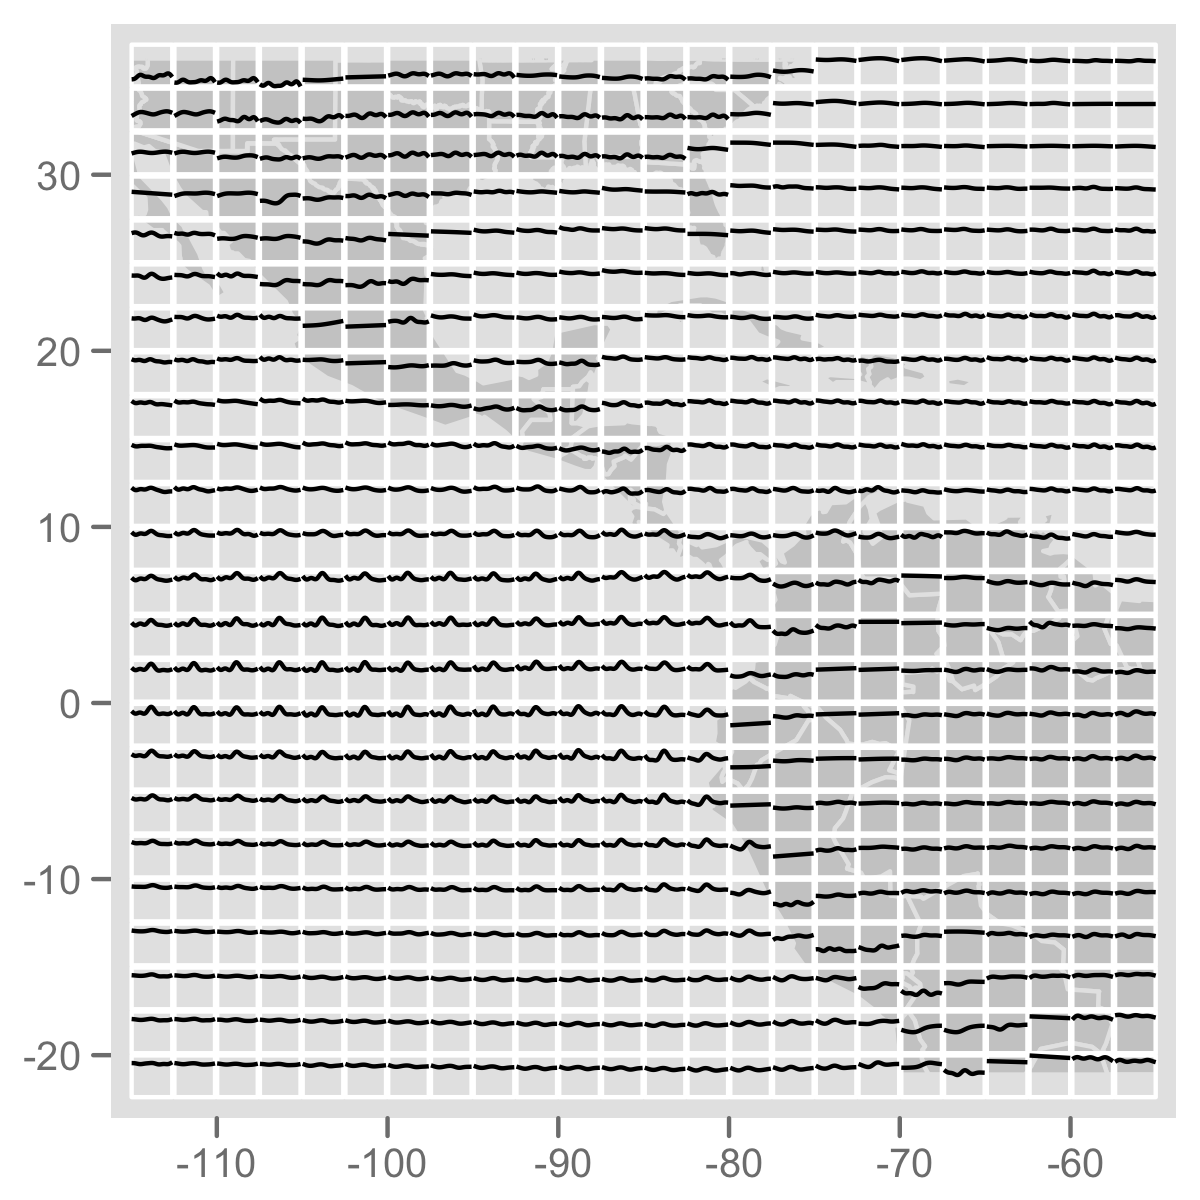
\includegraphics[width=0.5\linewidth]{month-rescale-none}%
  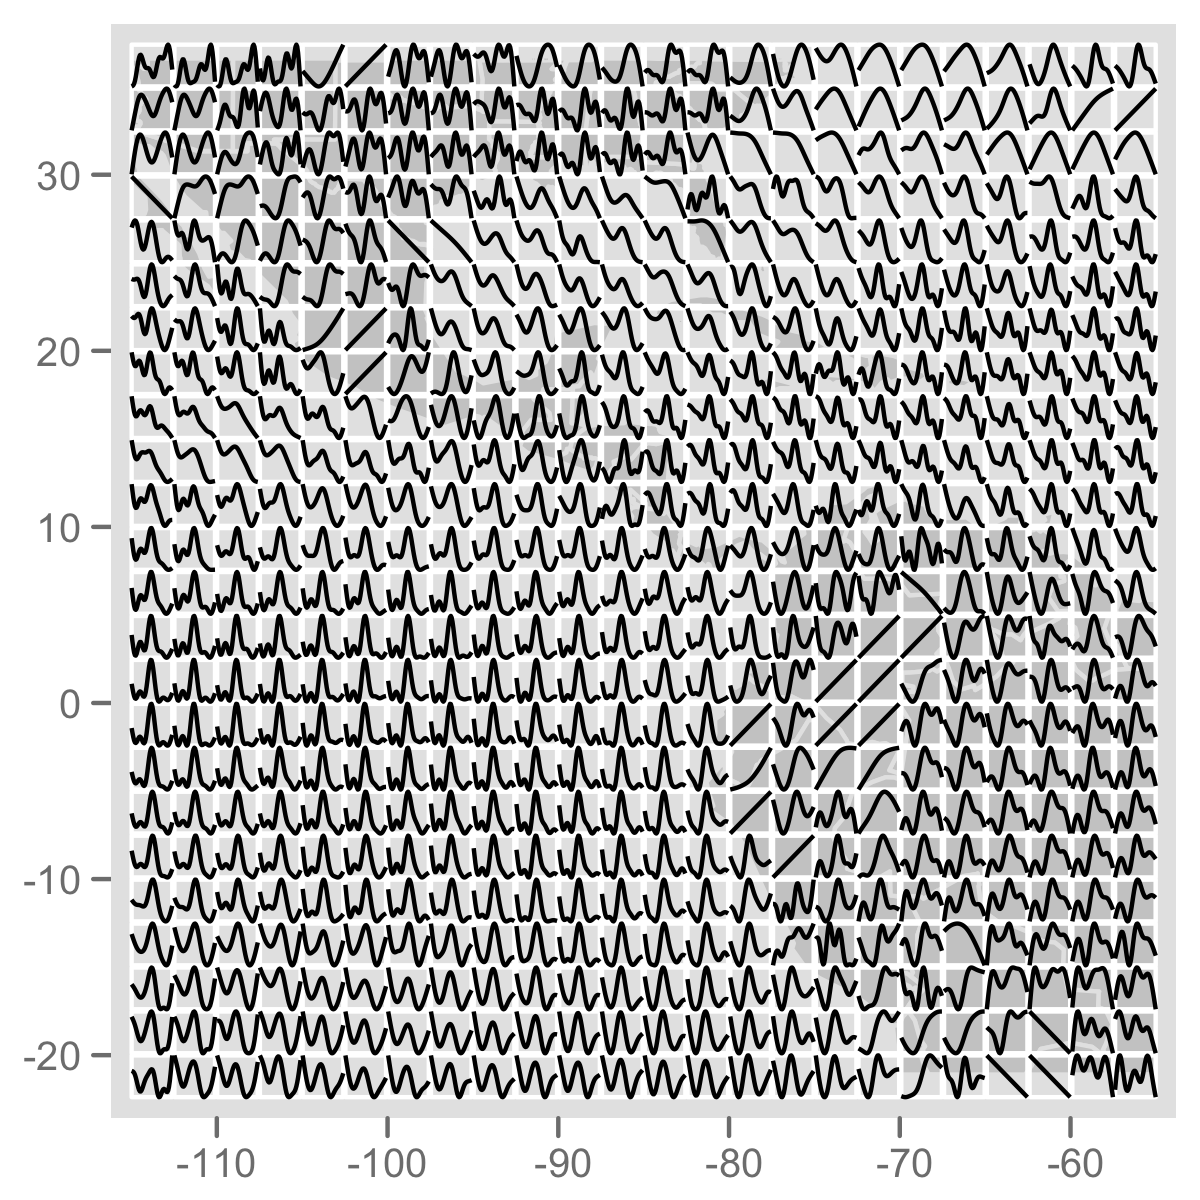
\includegraphics[width=0.5\linewidth]{month-rescale01}

  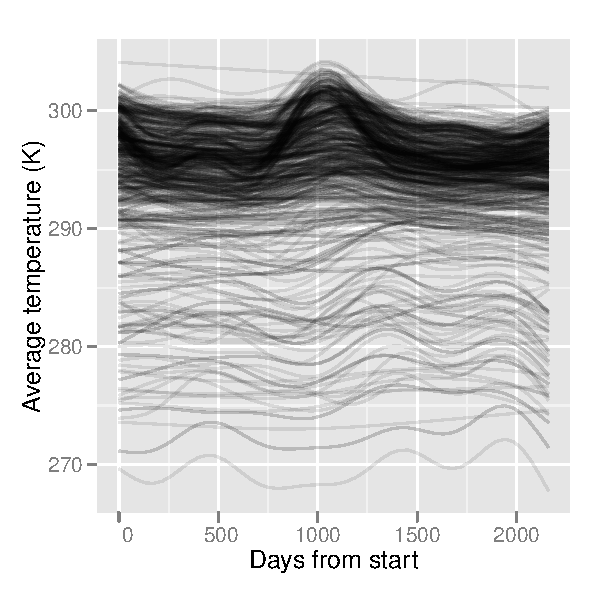
\includegraphics[width=0.33\linewidth]{month-rescale-legend}

  \caption{Glyph-map using predicted daily temperature values from a generalized additive model fit, where seasonality has been extracted: globally scaled (top left), locally scaled (top right). (Bottom) Legend showing ranges of individual glyphs.}
  \label{fig:scaling}
\end{figure}

Other types of shifting and scaling can be useful:

\begin{itemize} \itemsep 0in

\item The mean and standard deviation (or robust equivalents) could be
  used to standardize values to common moments. This may lead to some
  glyphs overlapping neighbors.
  
   \item Scaling to maximum 1 (but leaving the minimum unchanged) can help
  emphasis the relative shape.

  \item Shifting the values at each location to have mean zero places more
  focus on the trend. This is particularly important for the star glyphs,
  where differences in the average value lead to unintuitive patterns in the
  resulting glyphs.

\end{itemize}

Note that the use of local scales needs to be clearly marked. The viewer must realize that the scale is not relative and that big patterns in some locations might be just tiny, nugatory effects. To indicate this on the locally scaled data plots, one can use an additional aesthetic, like color, to encode the range of original scale. This is illustrated in Figure~\ref{fig:scaling-col}. In the encoding, emphasis is placed on the locations with larger range, stronger effects: the line intensity is darker (left plot), and the background is lightened to provide greater contrast (right plot) drawing the eye to these regions. 

\begin{figure}[htbp]
 \centering
 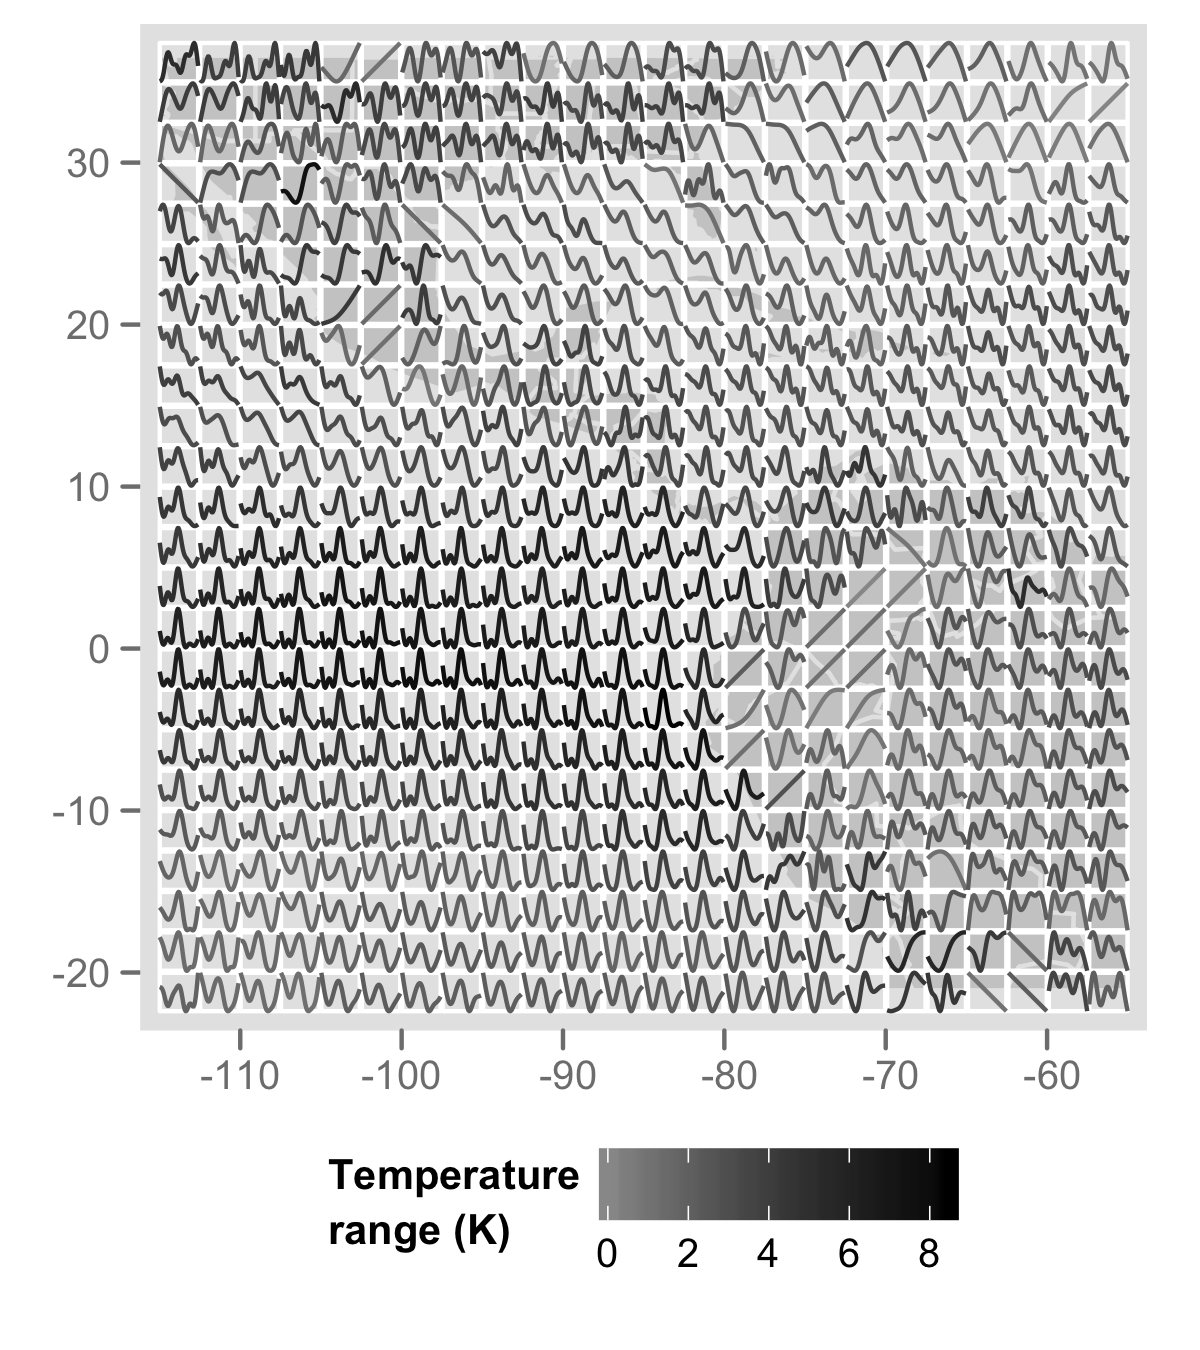
\includegraphics[width=0.5\linewidth]{month-rescale01-col}%
 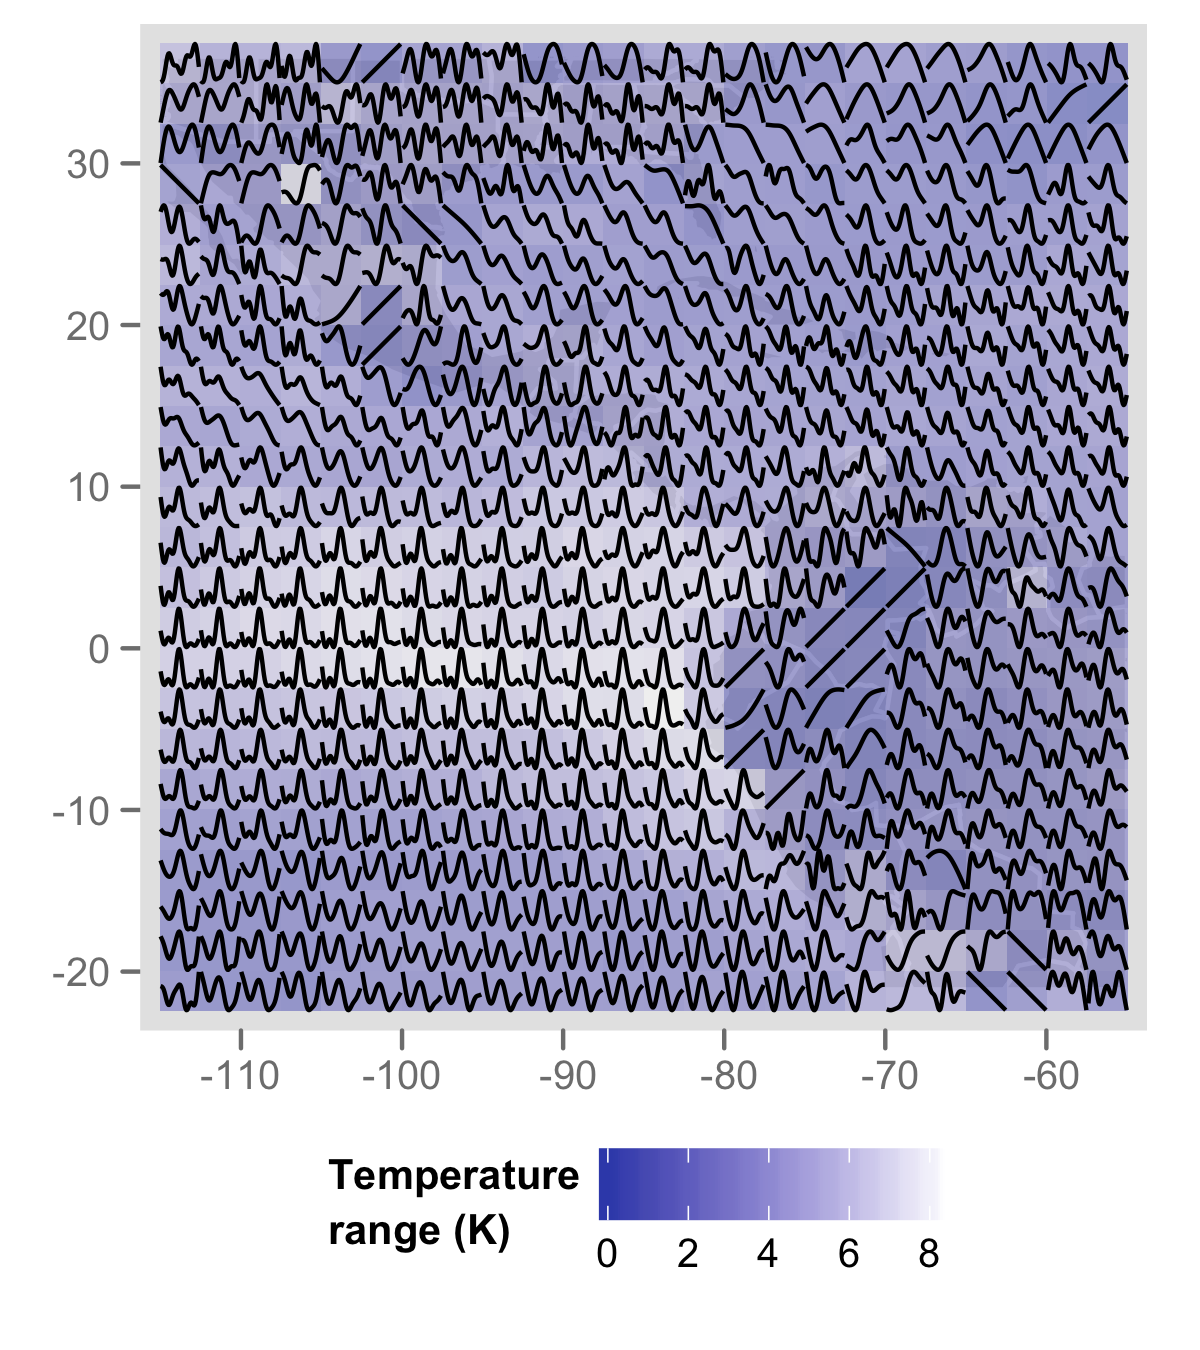
\includegraphics[width=0.5\linewidth]{month-rescale01-fill}
 \caption{Adding intensity and color to scaled plots. Here each location has been scaled to range $[0, 1]$ and color mapped to the range of the original predictions. (Left) Range mapped to intensity (grey scale) of the line: pale locations have smaller effect, smaller range, than darker locations, stronger effect. (Right) Range mapped to fill color of grid box: blue boxes have smaller effects, and light boxes have larger effects. Shapes at all locations are visible, but attention is drawn to locations with lighter backgrounds, larger ranges, because of the higher contrast.}
 \label{fig:scaling-col}
\end{figure}

One more important point: if a model summary is displayed in the glyph-map, as discussed in the following section, it may be important to force the scale to that of the original data. The range of predicted values is typically much smaller than the raw data, so angles of slopes are increased, giving an inaccurate sense of a stronger effect.  

\section{Large data and models}
\label{sec:large-data}

Climate data are usually large: many locations in space, and many points in time, which can make it arduous to work with computationally. The glyph-map calculations are as efficient as possible computationally, being linear in the number of spatial locations. It is possible that the calculations could also be parallelized for massive amounts of climate model data. Visualizing large data also hits a perceptual boundary.  There is a limit to the resolution of human visual system \citep{Kr12} which will prevent perfect perception of large spatial domains or seasonality of many years of data. Exploring large data requires reducing it to a resolution that can be reasonably absorbed visually.


Figure~\ref{fig:gistemp-raw} shows the glyph-map for the GISTEMP data set, which is more realistically sized than the EXPO data. Glyphs at each location represent temperature from 1880--2011, starting with Jan 1880 at 12 o'clock and proceeding clockwise to 2011 at 11:59. The most important feature to notice is the pattern of missing values. Most glyphs do not complete the full circle, typically missing points between 12 and 1, suggesting missing values in the earliest part of the data. Another important feature is variability, shown by the thickness of the circle. Some locations, particularly in the north and western mountain region, have large variations in temperature. 

\begin{figure}[htbp]
  \centering

  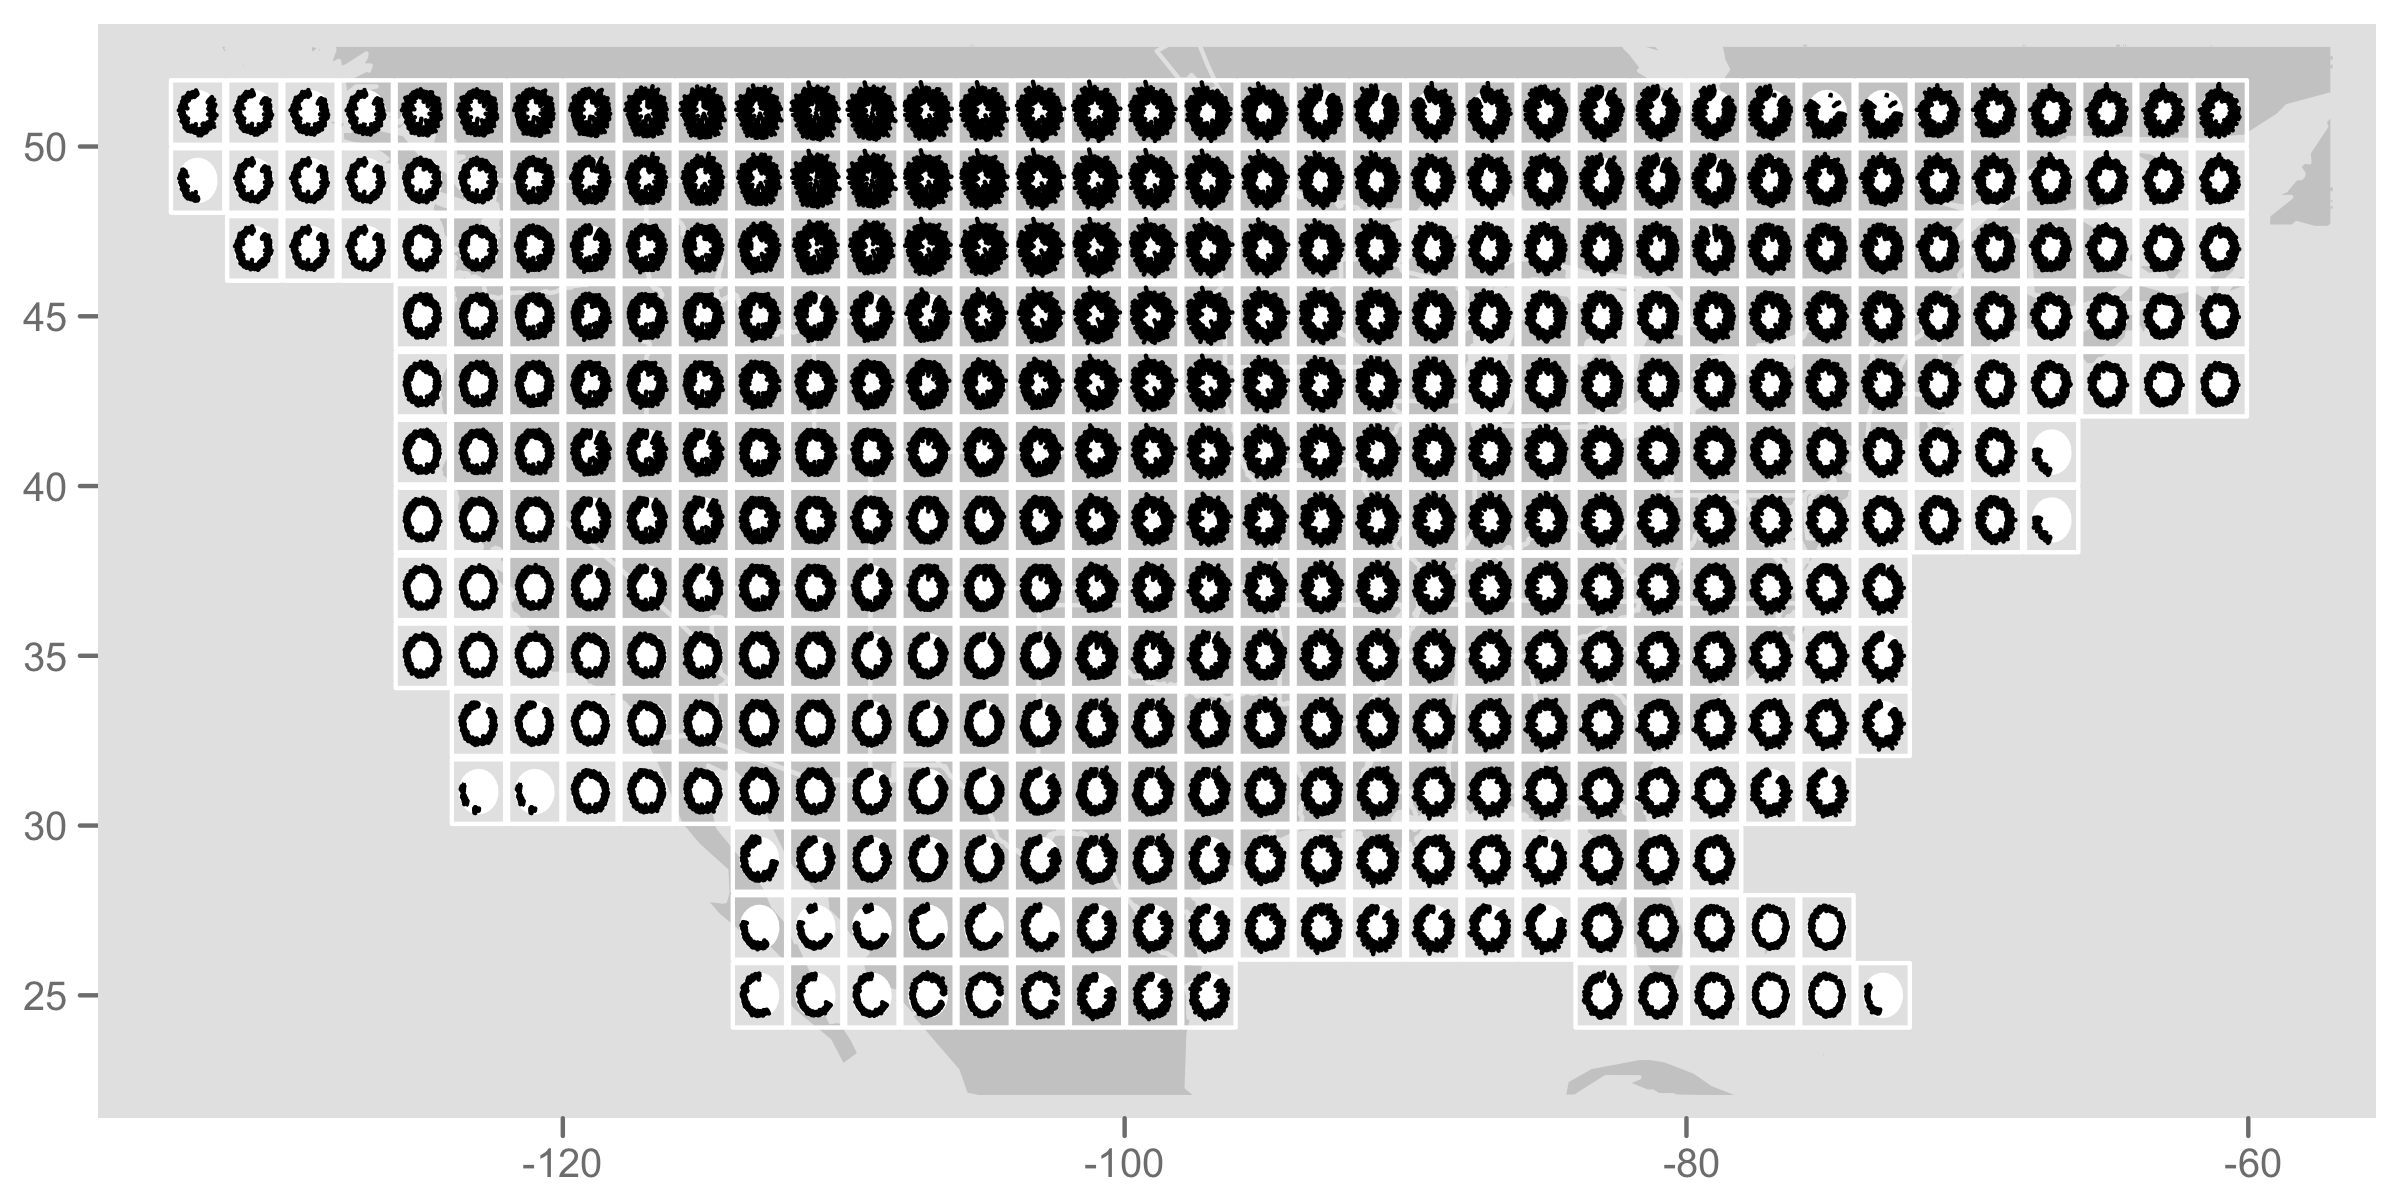
\includegraphics[width=1\linewidth]{gistemp-polar-raw}

  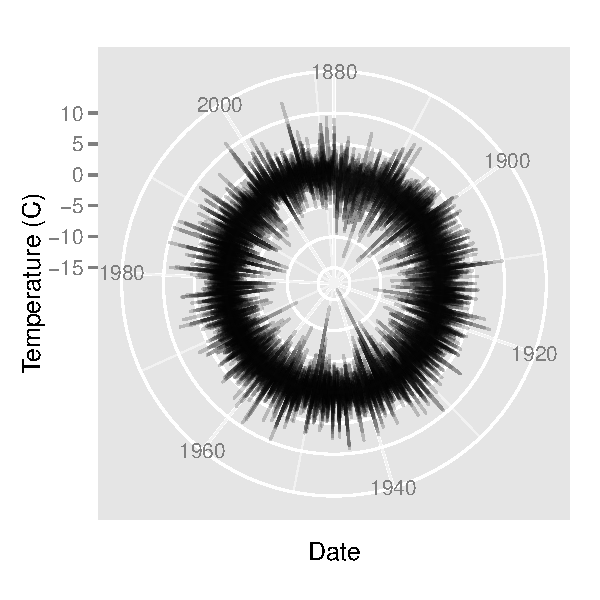
\includegraphics[width=0.33\linewidth]{gistemp-polar-legend}

  \caption{(Top) Glyph-map of raw temperature anomaly data (GISTEMP), from 1880-2011. Gaps in the full circle indicate missing values, and thickness of the circle indicates more variability in the measurements.  (Bottom) Legend showing temperature and temporal ranges of individual glyphs.}
  \label{fig:gistemp-raw}
\end{figure}

The raw data shows us missing values and gives some sense of variability, but gives no information about long-term trend. Statistical models are useful for pre-processing climate data, to decompose data into long-term trend, seasonal effects and error, which is vital for making the problem both computationally and visually tractable. Trend is examined by fitting a linear model to each location and displaying predicted values in Figure~\ref{fig:gistemp-pred}. This plot shows long-term (de-seasonalized) temperature trends for 1950--2010. (The reduced time period is used to eliminate the influence of the missing data values in early years.) Most locations have increasing temperature over this time period. Only a few locations show a decline, and these few locations tend to be different from their neighbors, and on the edge of the data collection region, indicating that there might be isolated data problems. The rate of increase differs across regions: steeper inclines in the north and western mountain regions and across the Great Lakes, and flatter inclines in the southeastern USA.

\begin{figure}[htbp]
  \centering
  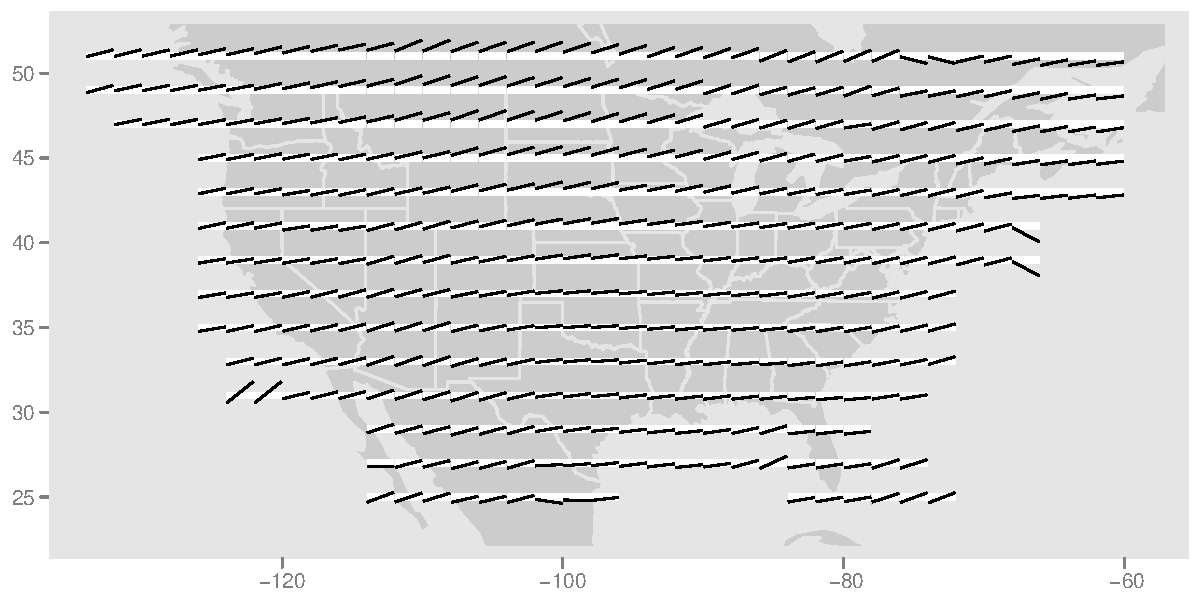
\includegraphics[width=1\linewidth]{gistemp-pred}

  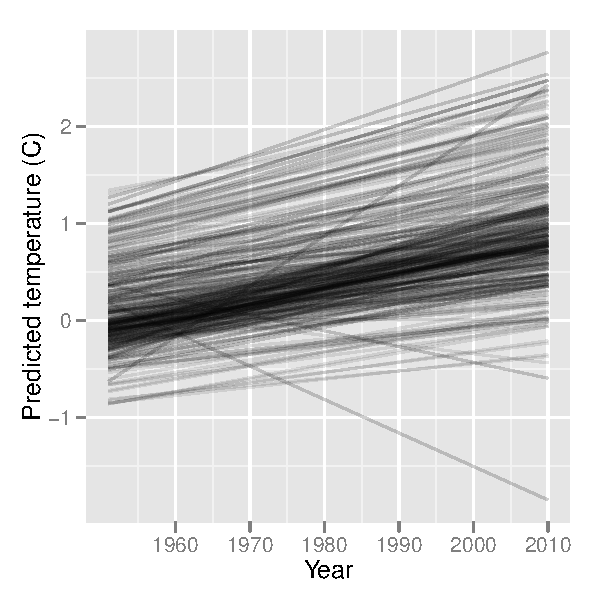
\includegraphics[width=0.33\linewidth]{gistemp-pred-legend}
  
  \caption{(Top) Glyph-map of predicted temperature anomaly data
    (GISTEMP), for the reduced period 1950-2010. Increasing
    trends can be seen over most of the USA, with varying degrees of
    increase. Some isolated locations exhibit steep declines, and
    inclines, perhaps indicative of some isolated data problems. Note
    that, the reference lines are straight, but they look curved
    because of the Z\"ollner optical illusion. (Bottom) Legend showing
    temperature and temporal ranges of individual glyphs.}
  \label{fig:gistemp-pred}
\end{figure}

\section{Non-gridded data}~\label{sec:irregular}

Regularly gridded spatial data helps with the perception of structure, because it helps to provide the reference frames upon which to make comparisons among the icons. When spatial locations are not on a regular grid, some difficulties arise. In this situation it is not clear what the scale of icons should be, as there is no regular spacing. Some locations may be close to each other which would generate icons that overlap. 

\subsection{Non-rectangular grids}

Glyph-maps work best when displayed in the coordinate system in which the grid is rectangular and regular.  For example, the GISTEMP grid is 2$^o$ square and is displayed treating longitude and latitude as Cartesian coordinates in Figures~\ref{fig:gistemp-raw}, \ref{fig:gistemp-pred}.  For regularly gridded data, this results in icons that are rectangles of equal size.  It is often preferable to display maps as a projection of the geographical coordinates which preserves a property of interest, area for example. When a projection is desired, a choice needs to be made between applying the projection to the completed glyph-map, or to just the spatial locations.  When the completed glyph-map is projected the icons are no longer rectangles of the same size but they do retain their space filling property.  When applying a projection to the spatial locations and then constructing a glyph-map, the grid becomes irregular. 

\subsection{Irregular locations}
Figure \ref{fig:irregular} shows linear trends for monthly average surface temperature at stations in the USHCN data.  It illustrates three challenges in working with irregular locations: there is no natural choice for icon size, icons can potentially overlap, and comparisons rely more heavily on the reference guides.  The icon size was chosen manually for this plot, corresponding to 1$^o$ square in the geographical coordinates. 
\begin{figure}[htbp]
  \centering
  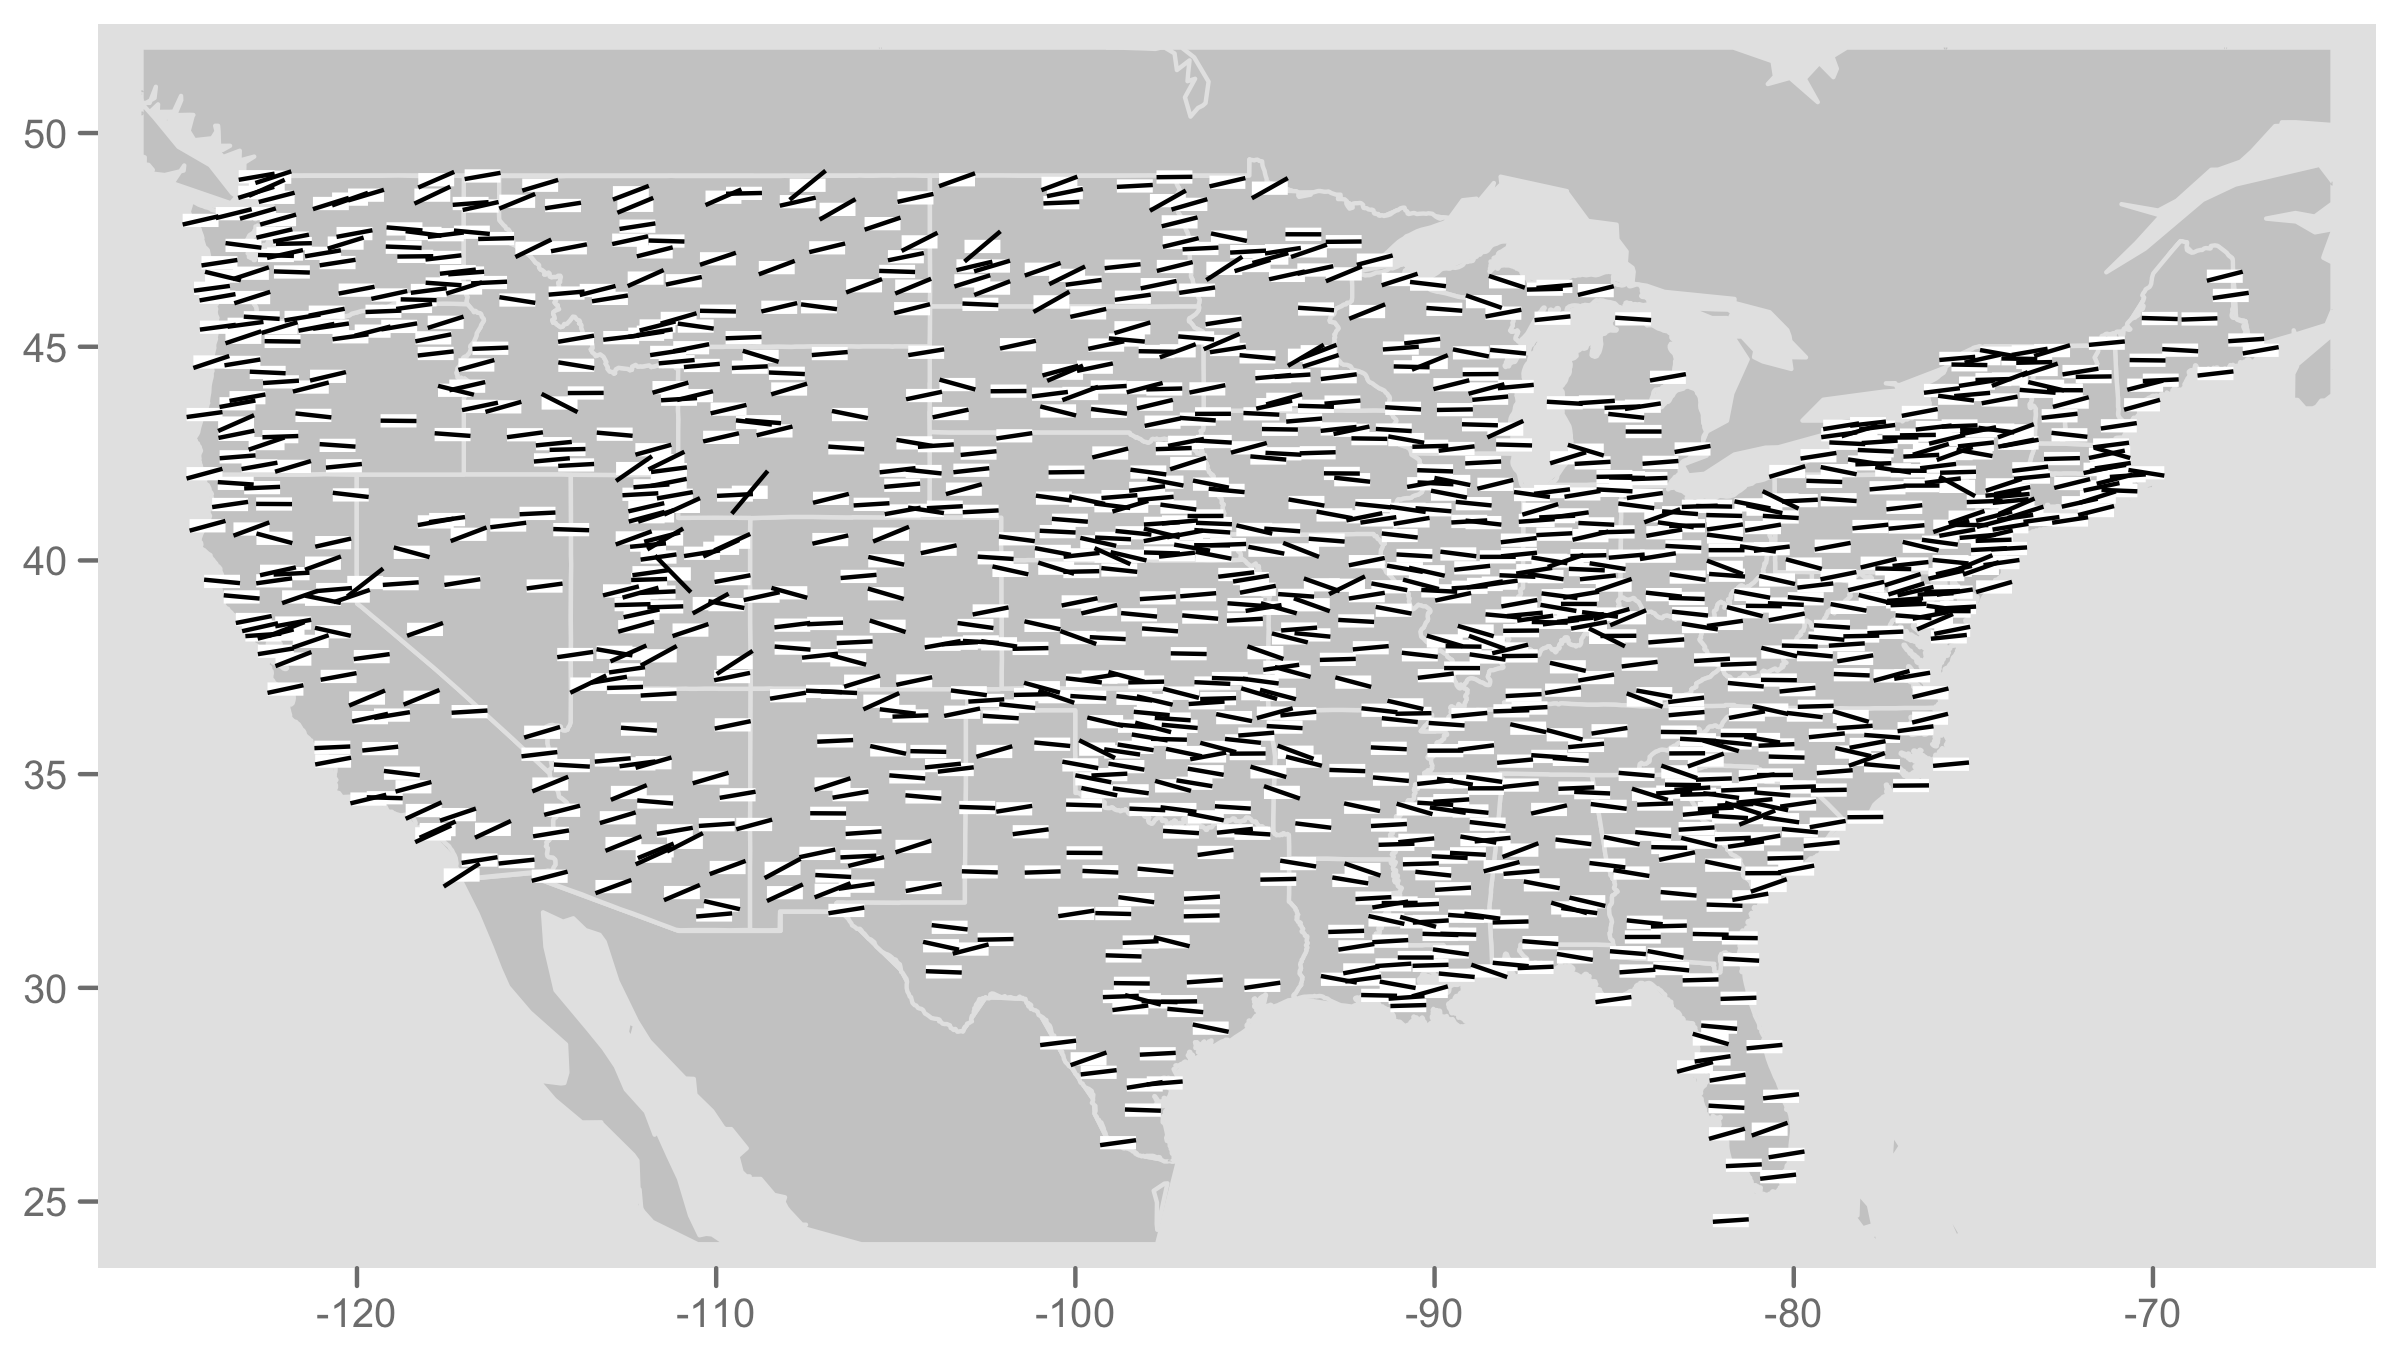
\includegraphics[width=1\linewidth]{usa-lin-overlap}%

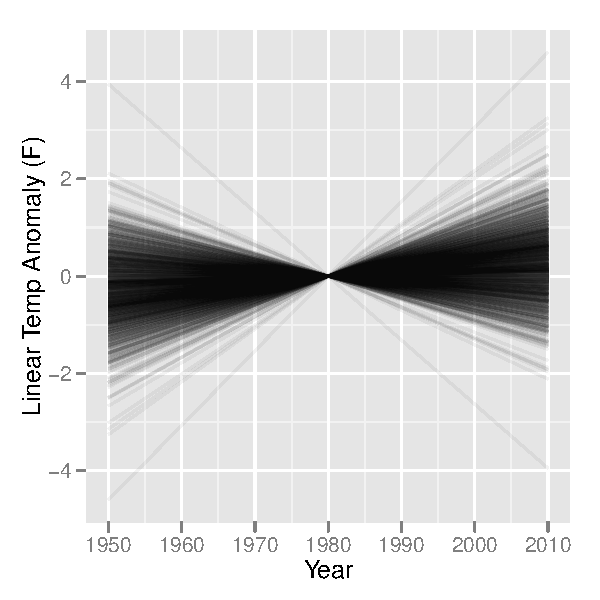
\includegraphics[width=0.33\linewidth]{usa-lin-legend}
  \caption{(Top) Glyph-maps of the linear trend in ground station temperature values, 1950--2010, for USHCN stations, illustrating three issues for irregularly gridded data: overlapping icons, no natural choice for icon size, and the disordered appearance making comparisons more difficult. Local centering, subtracting the location mean from the linear fit, is used as the variation in average temperature is of much greater magnitude than the variation in linear trend. (Bottom) Legend showing
    temperature and temporal ranges of individual glyphs. The local scaling is apparent here with all lines going through zero at the mean year. }  \label{fig:irregular}
\end{figure}
One solution to the overlapping problem is to zoom in on smaller regions. There is an interplay between icon size (in geographical units), area plotted (in geographical units) and plot size (in display units).  Icons need to be big enough to be readable on the display, but small enough to avoid overlapping.  Readability can be maintained and overlapping reduced by decreasing the icon size and simultaneously increasing the display size or decreasing the area plotted.

An alternative approach is to combine overlapping locations and plot a single summary icon.  In Figure \ref{fig:irregular-collapsed} nearby locations are collapsed to a single icon.  In the left panel each station still has an individual glyph but locations close to each other share a plotting area (note the multiple lines visible in some reference boxes). The right panel shows an example where glyphs are generated on aggregated data: the average trend for the collapsed locations is displayed.  To differentiate glyphs that involve summaries of more than one location, heavier lines (barely visible) indicate at least two locations that have been averaged.  The aggregation of spatial locations to a single summary can be misleading.  The sensitivity of analyses to the scale and configuration of aggregation is described by the  modifiable areal unit problem (\cite{Openshaw:1984kx, Fotheringham:1991uq}). In this type of glyph-map the scale of aggregation is determined, rather arbitrarily, by the icon size. This dependence of visual inferences on the icon size is undesirable.  The ability to interactively modify icon size, and zoom quickly to disaggregate locations would go some way to alleviating the problem.


\begin{figure}[htbp]
  \centering
  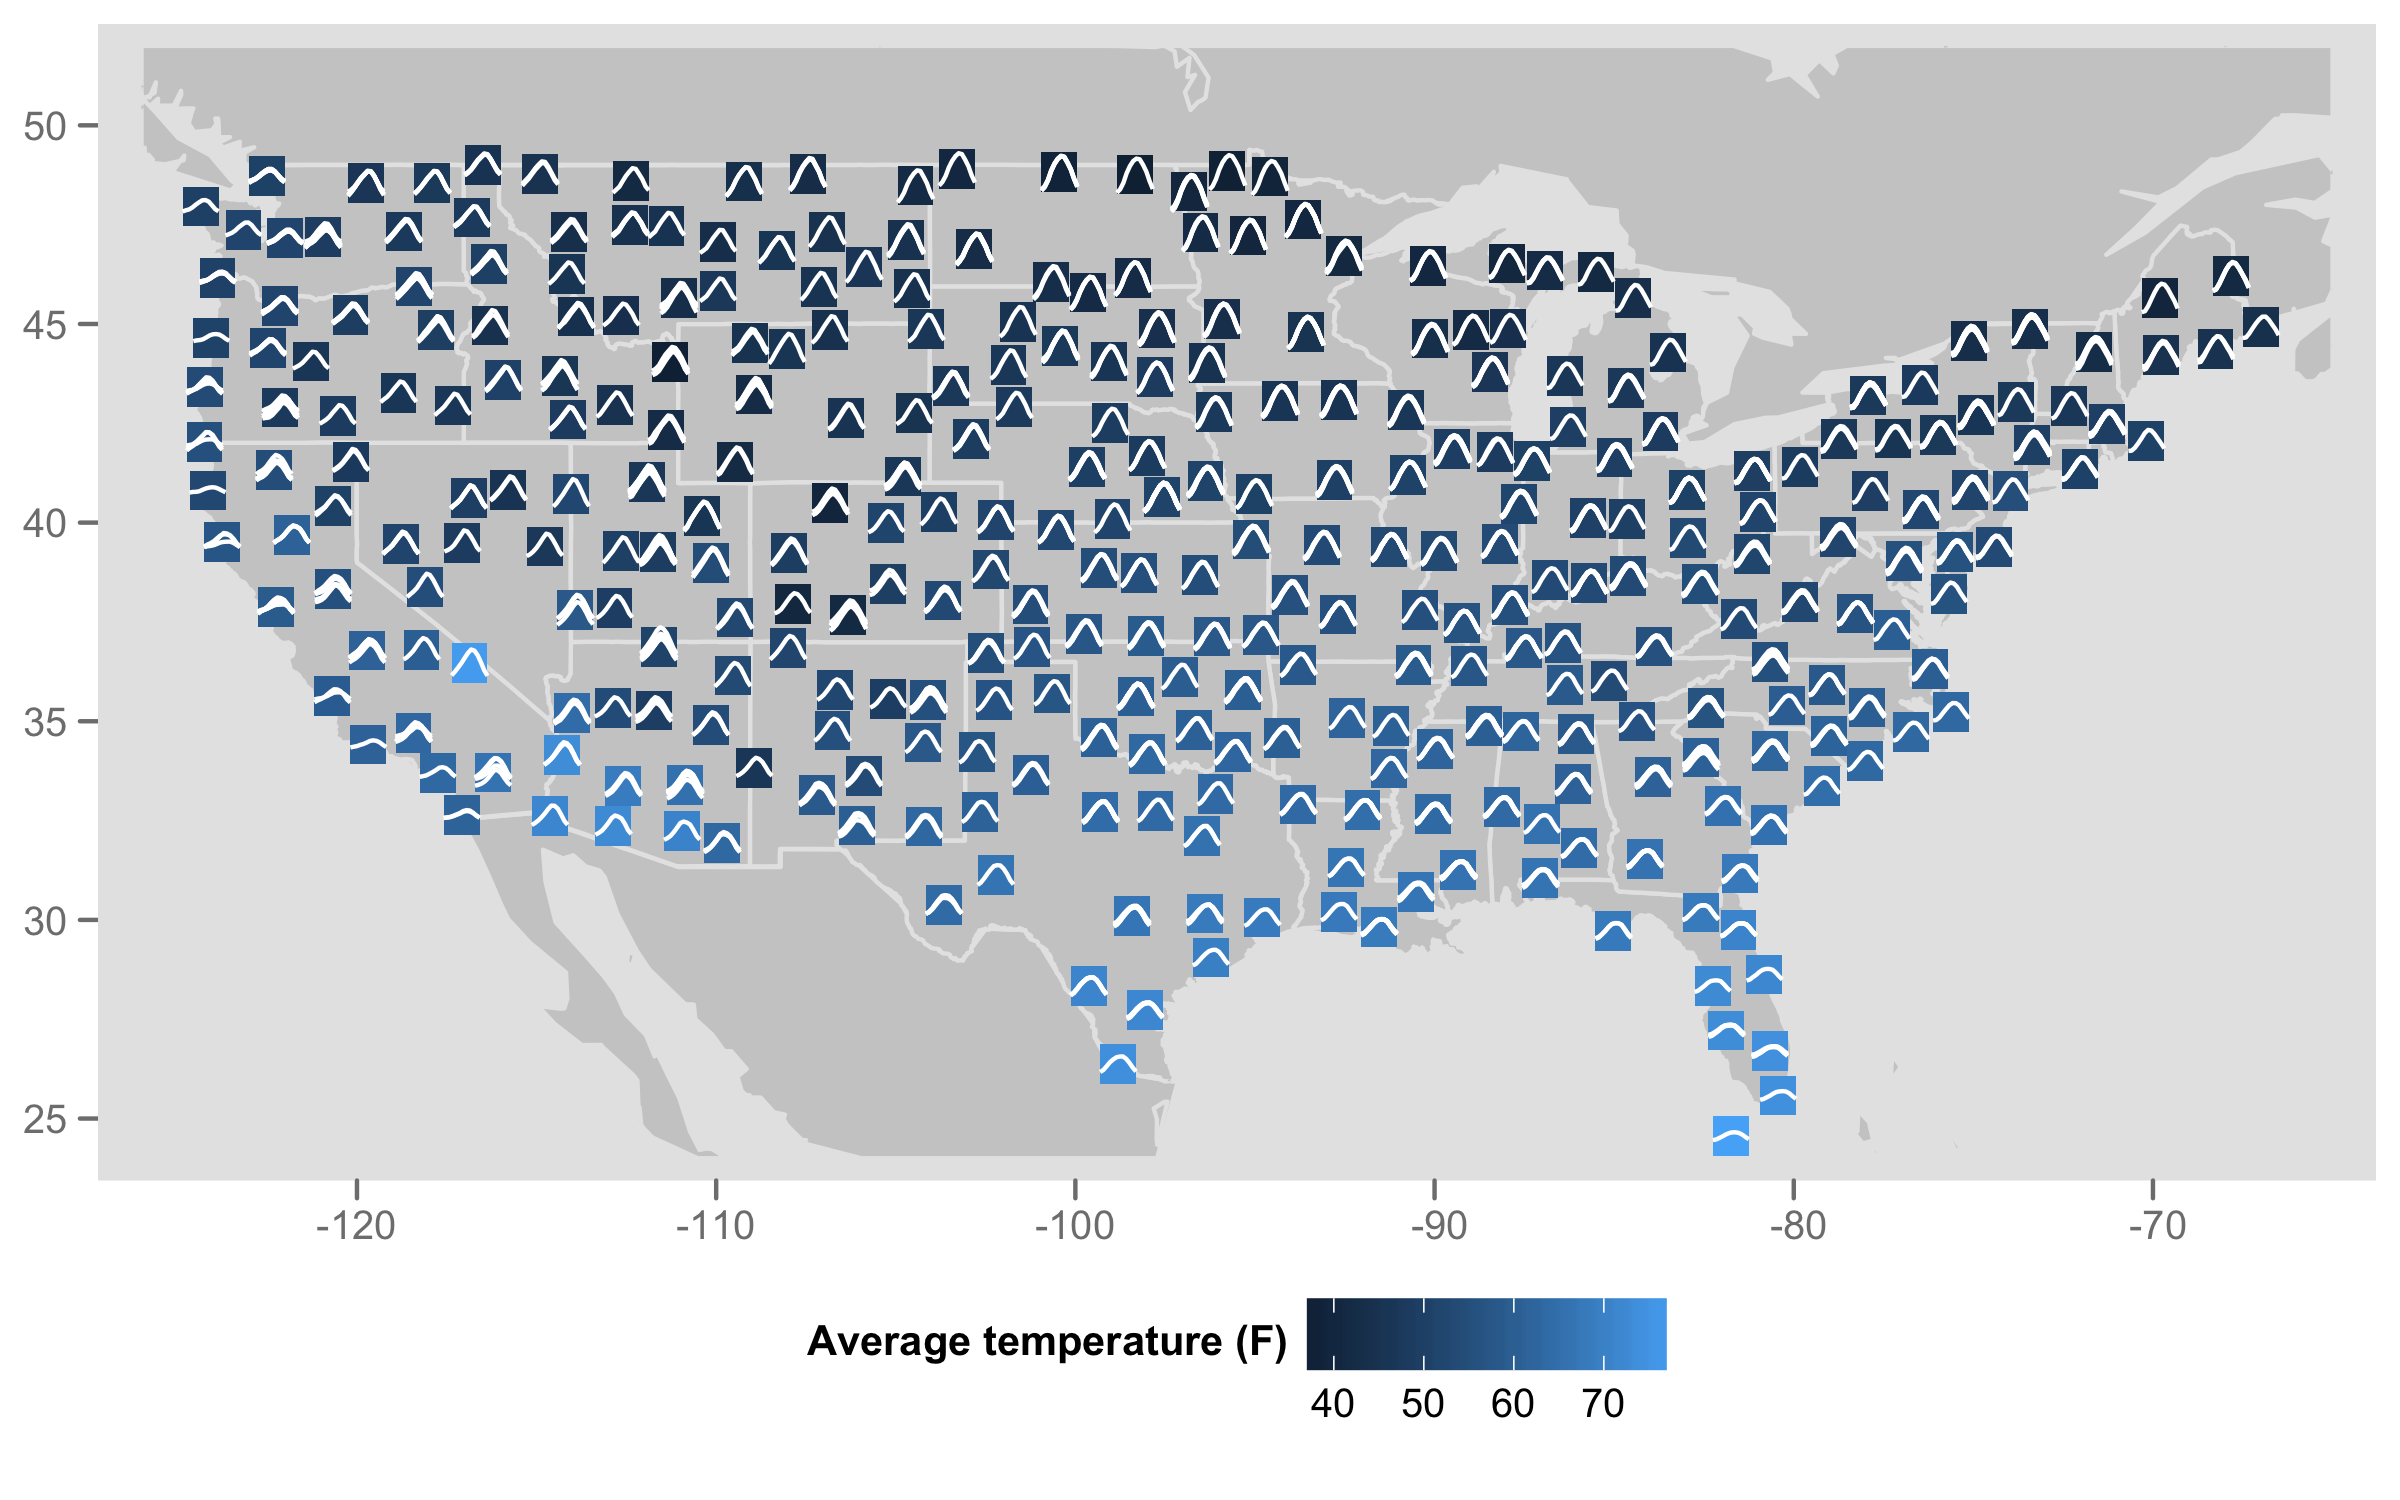
\includegraphics[width=0.5\linewidth]{usa-season-collapsed}%
  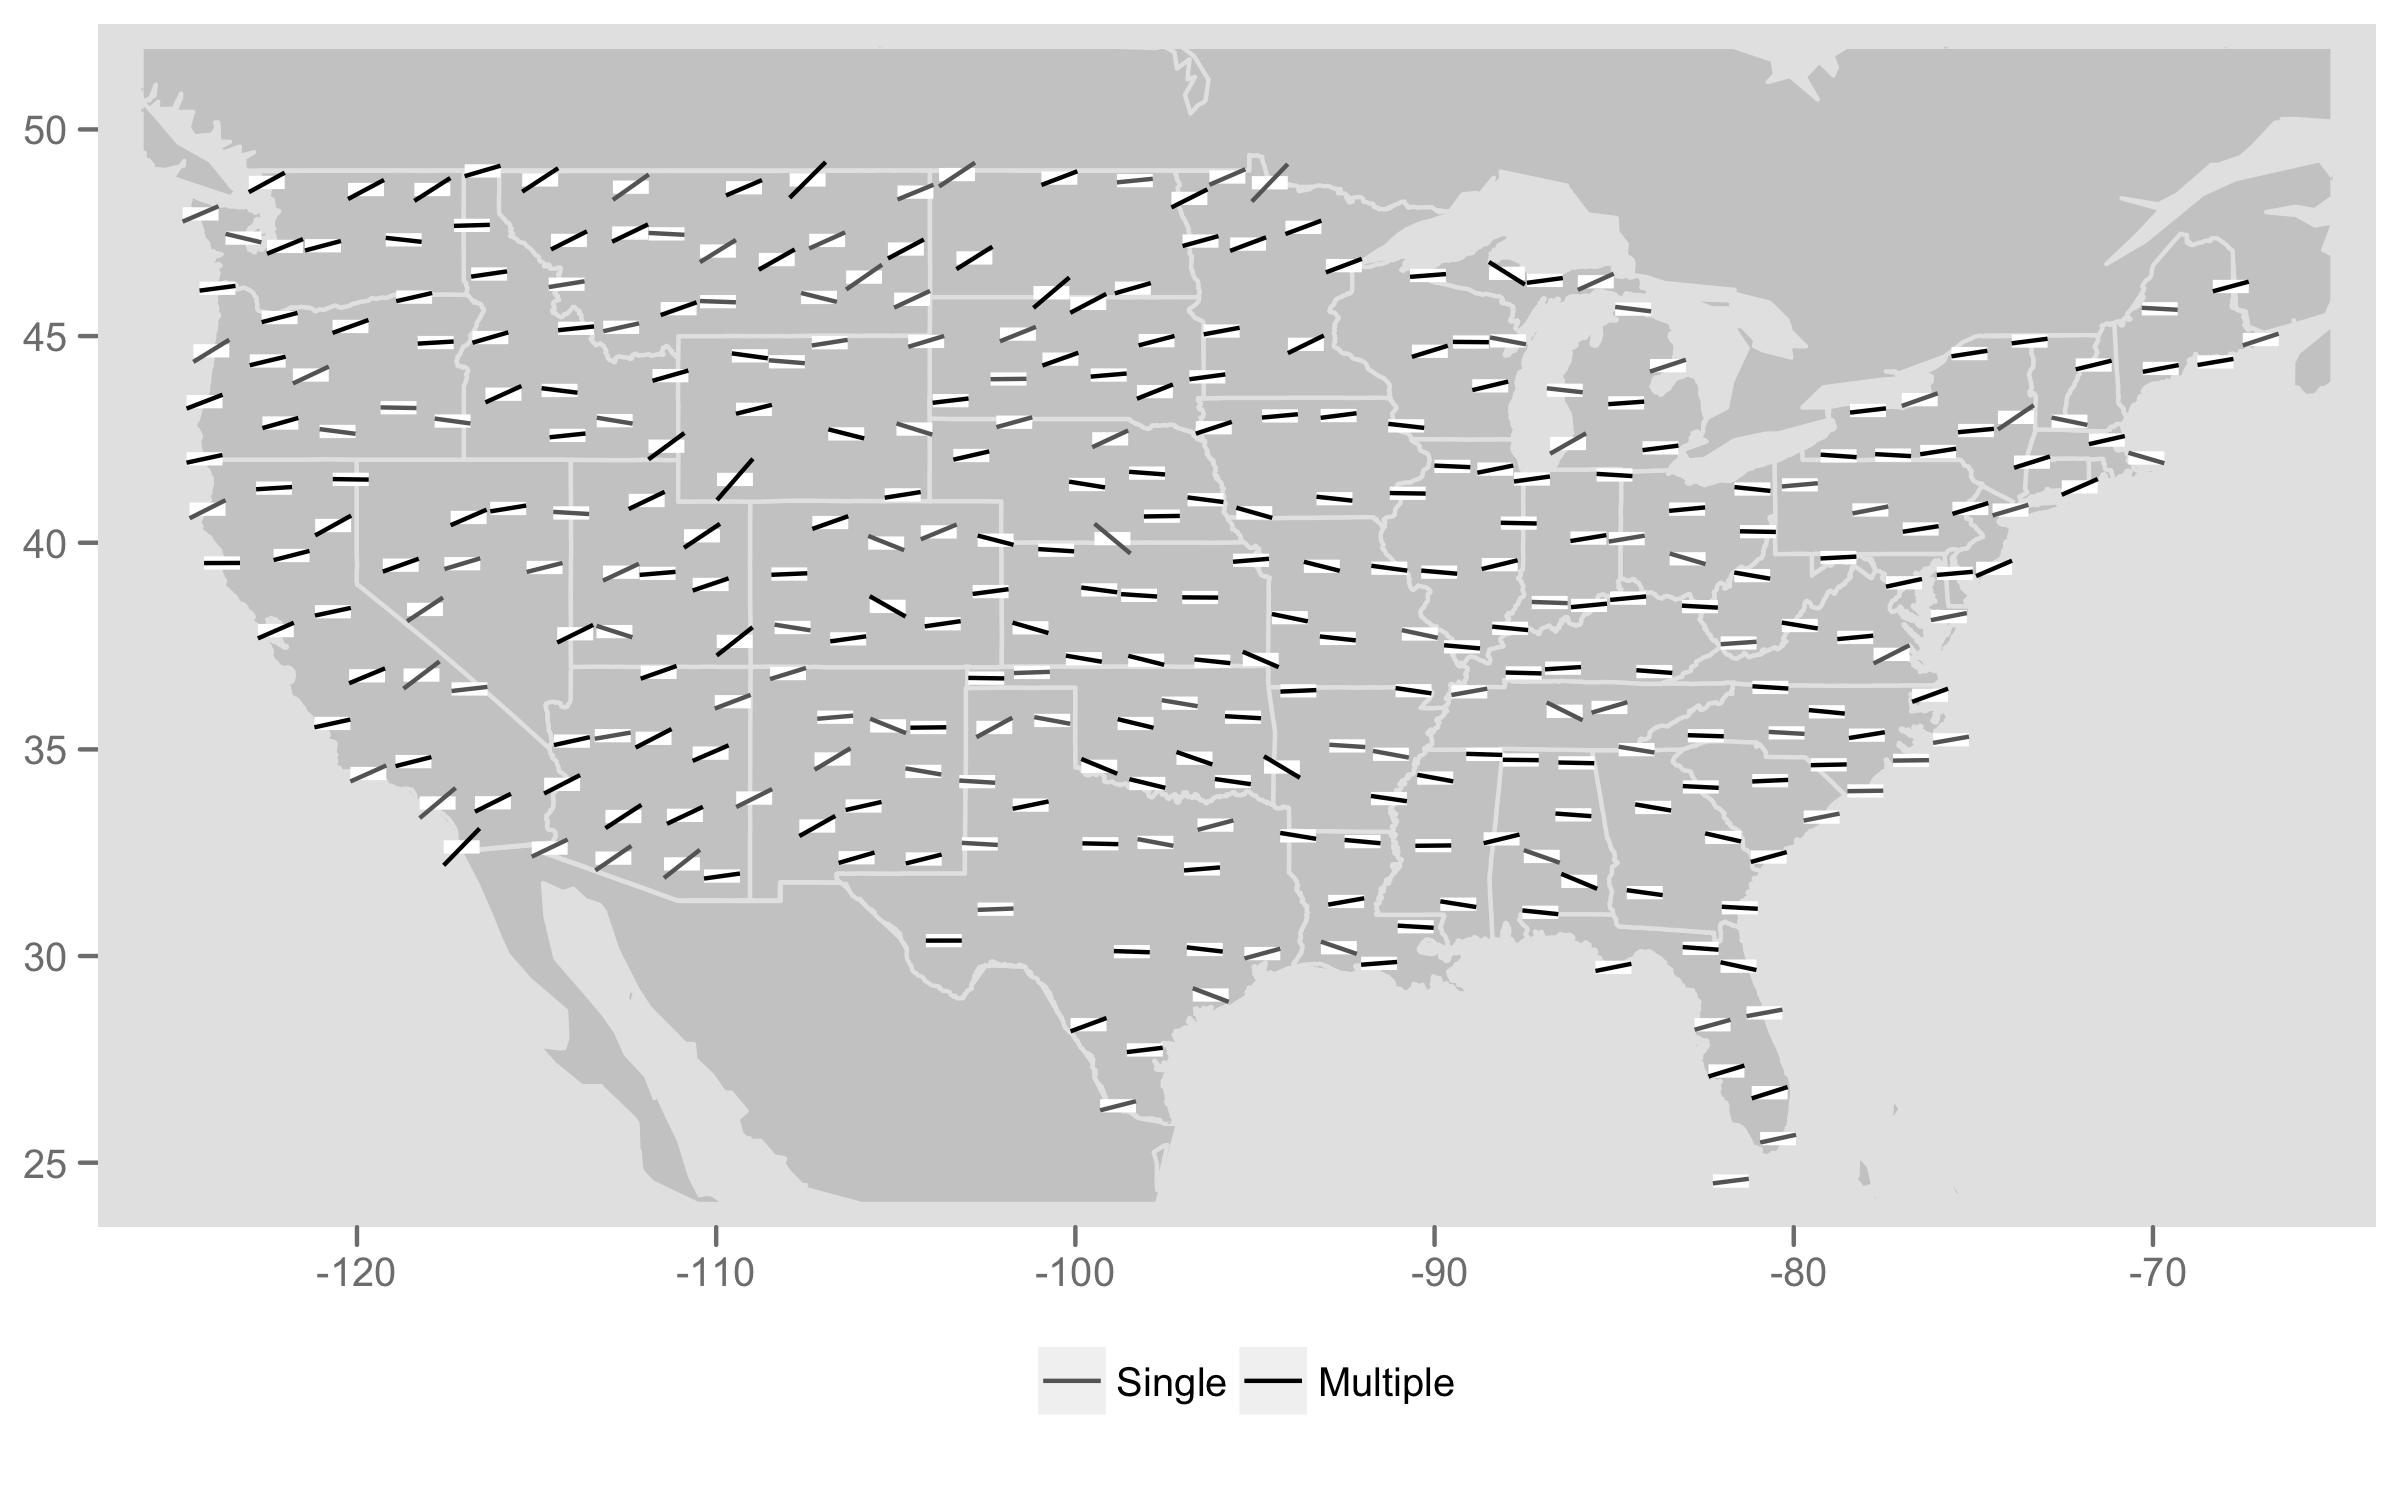
\includegraphics[width=0.5\linewidth]{usa-lin-collapse}%

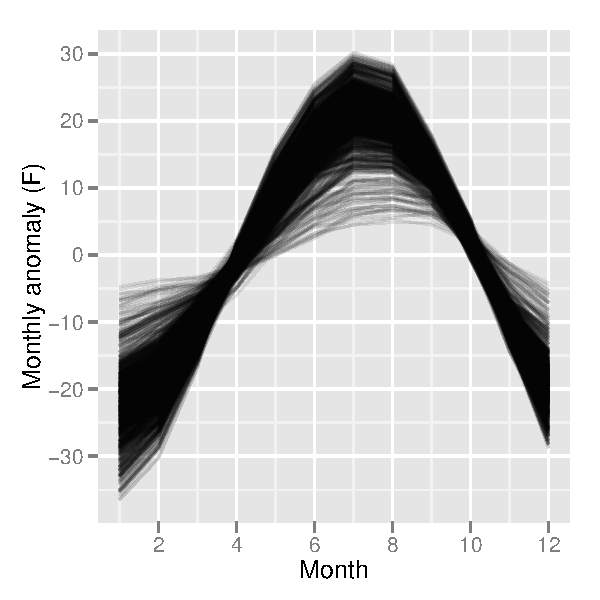
\includegraphics[width=0.20\linewidth]{usa-season-legend}\hspace{2in}%
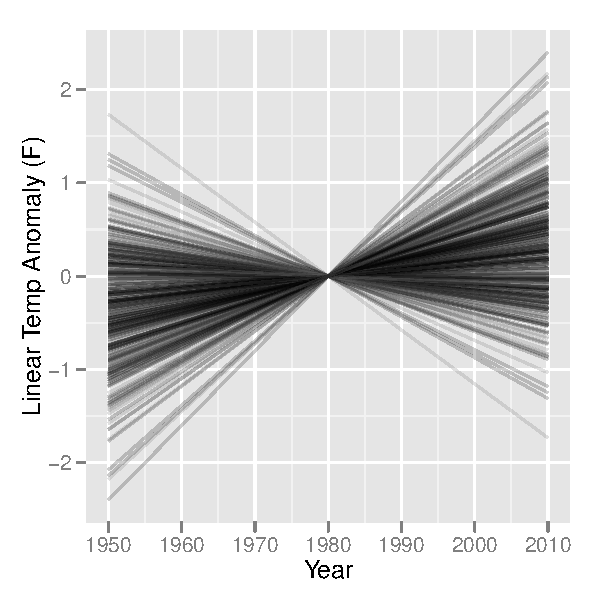
\includegraphics[width=0.20\linewidth]{usa-lin-collapse-legend}
  \caption{Glyph-maps of seasonal patterns (top left) and linear trends (top right) of USHCN stations, 1950--2010.  Nearby stations whose icons would overlap have been collapsed.  Each location has a glyph in the seasonal plot and color of the tiles corresponds to the average temperature of the locations.  Heavy lines in the linear trend plot correspond to average trends over more than one location. (Bottom) Legends showing scale of glyphs.} 
  \label{fig:irregular-collapsed}
\end{figure}

In both of the examples where locations have been collapsed, the icon locations still represent an actual geographic location of collected data, albeit including data from up to an icon-width away.  An alternative way to combine stations is to round locations to the icon size, as done in Figure \ref{fig:irregular-grid}. This produces a regular grid with the advantage of easier perception of structure \citep{Kr12b}. (Figure 9.12 of \citet{IPCC} uses a regular gridded time series over a spatial domain to illustrate temporal patterns in climate change data.) It hides the irregular nature of the locations, though, and a complication is that icons may end up centered over nonsense places, such as land measurements in the ocean.  

\begin{figure}[htbp]
  \centering
  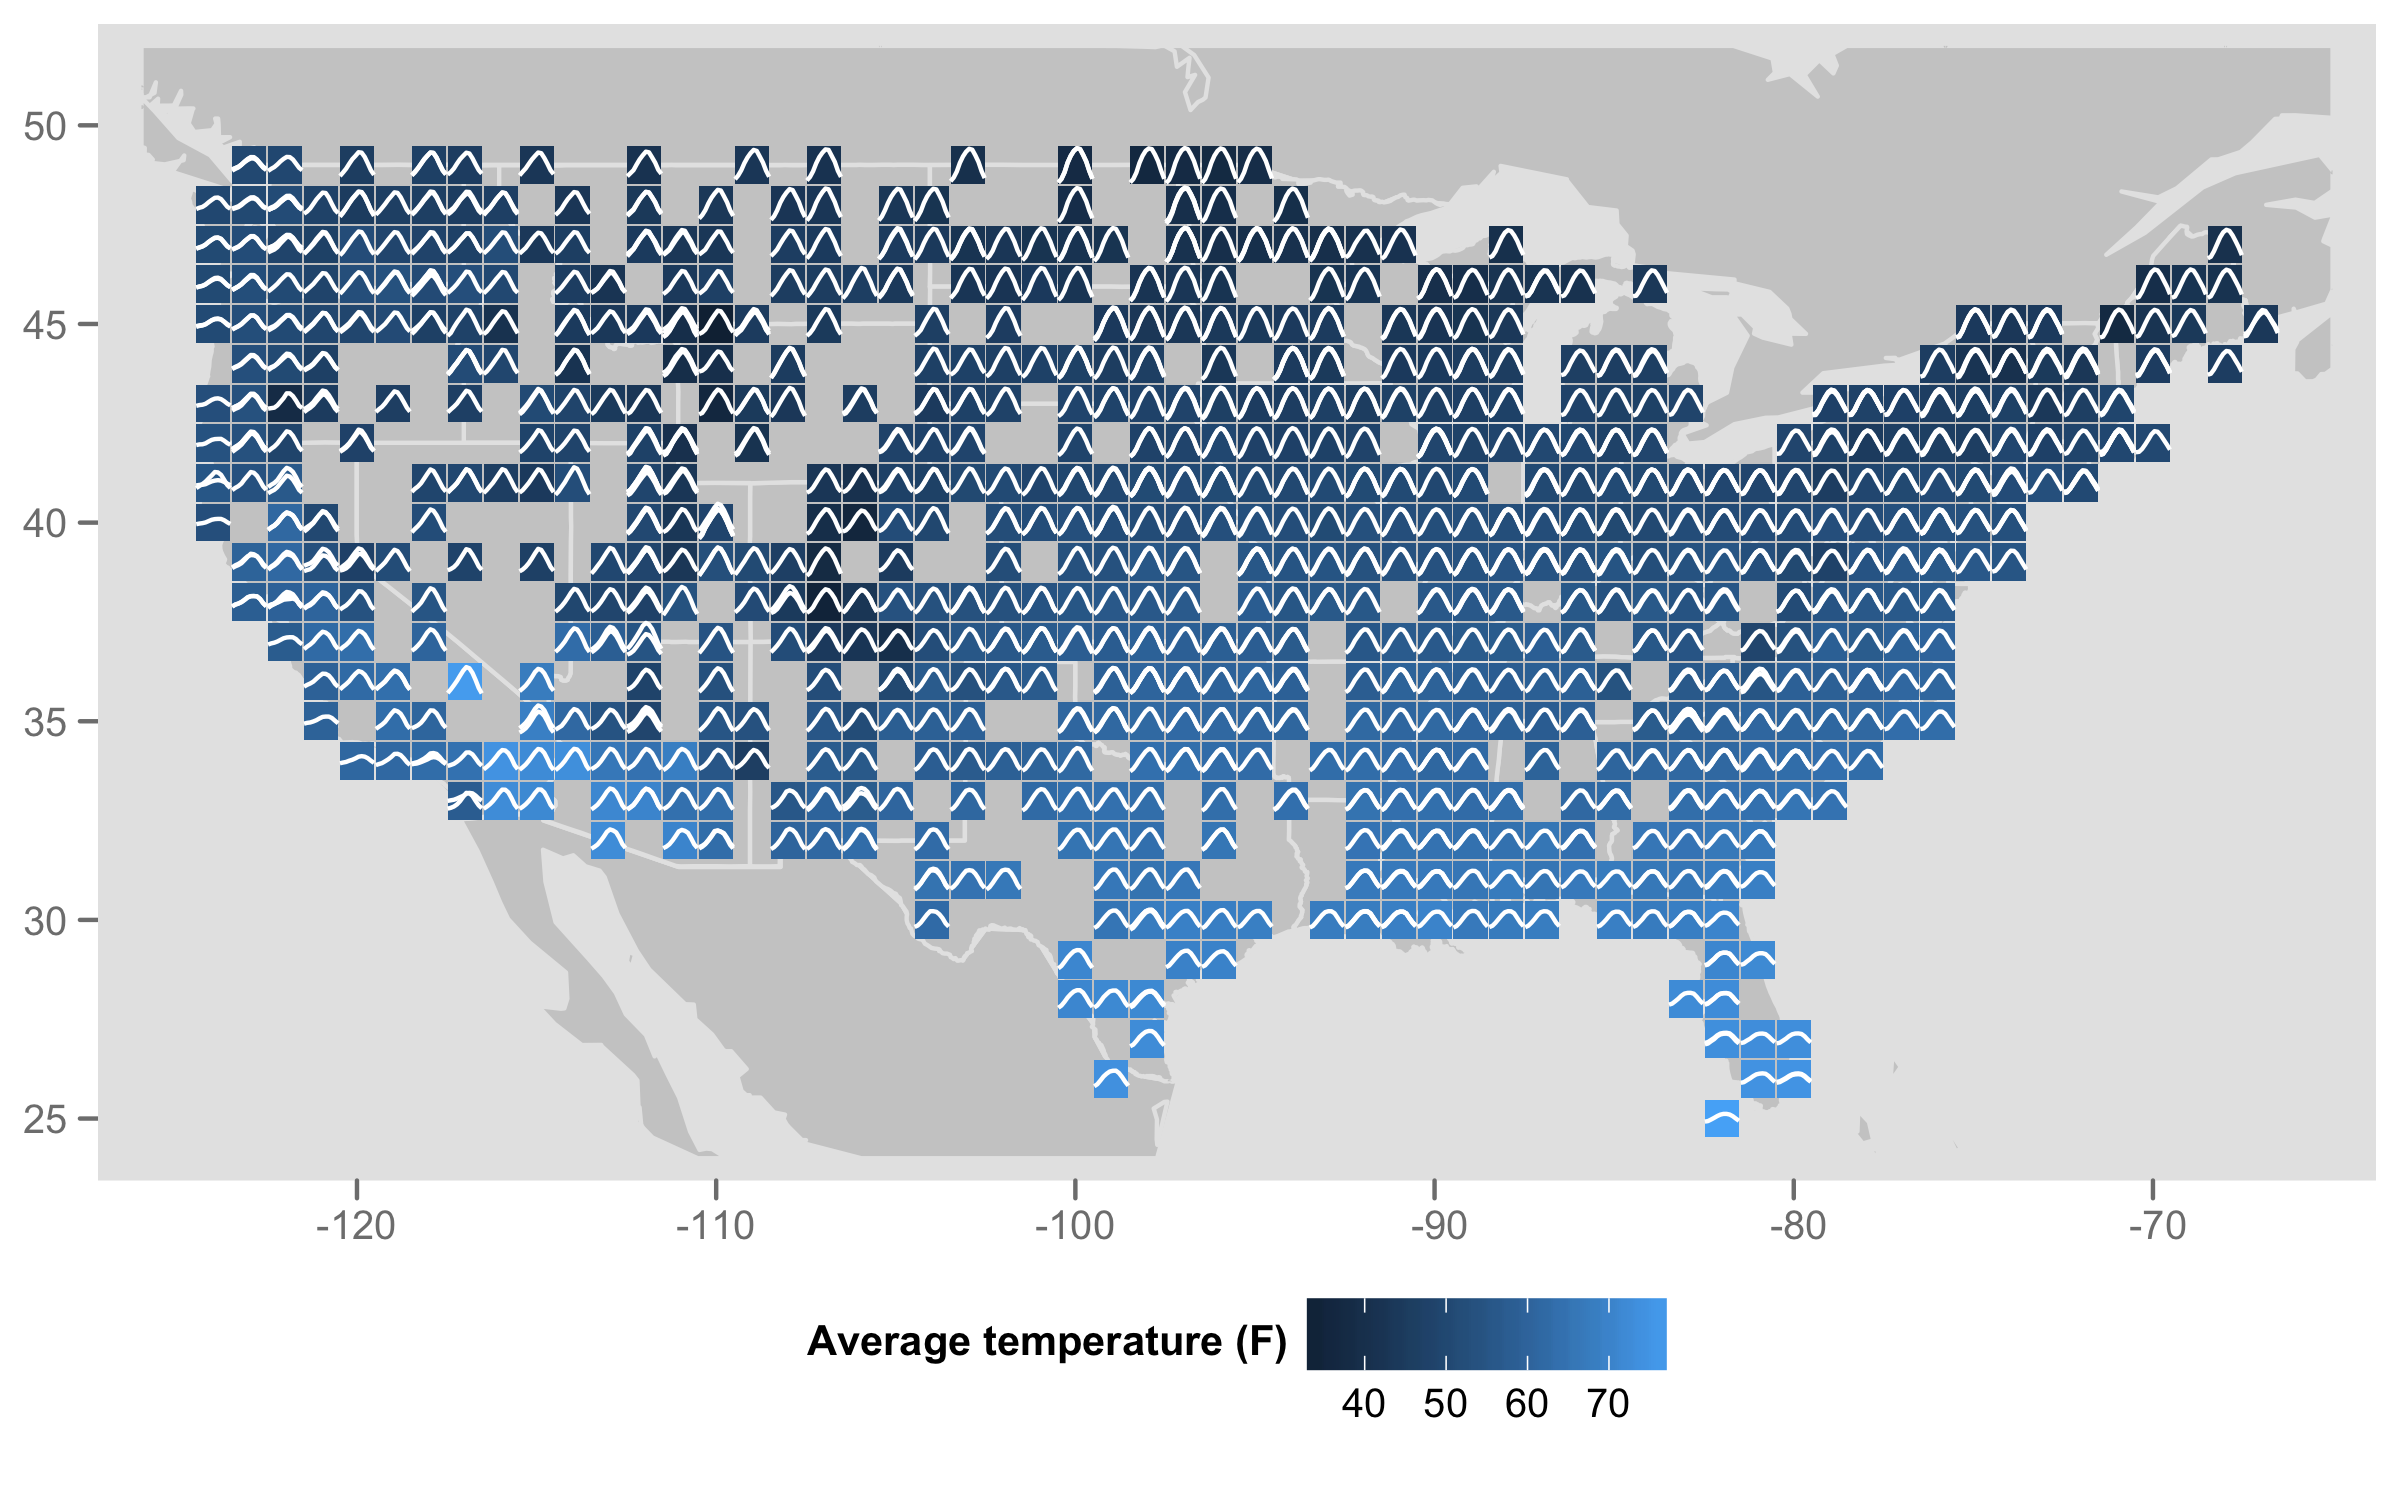
\includegraphics[width=0.5\linewidth]{usa-season-grid}%
  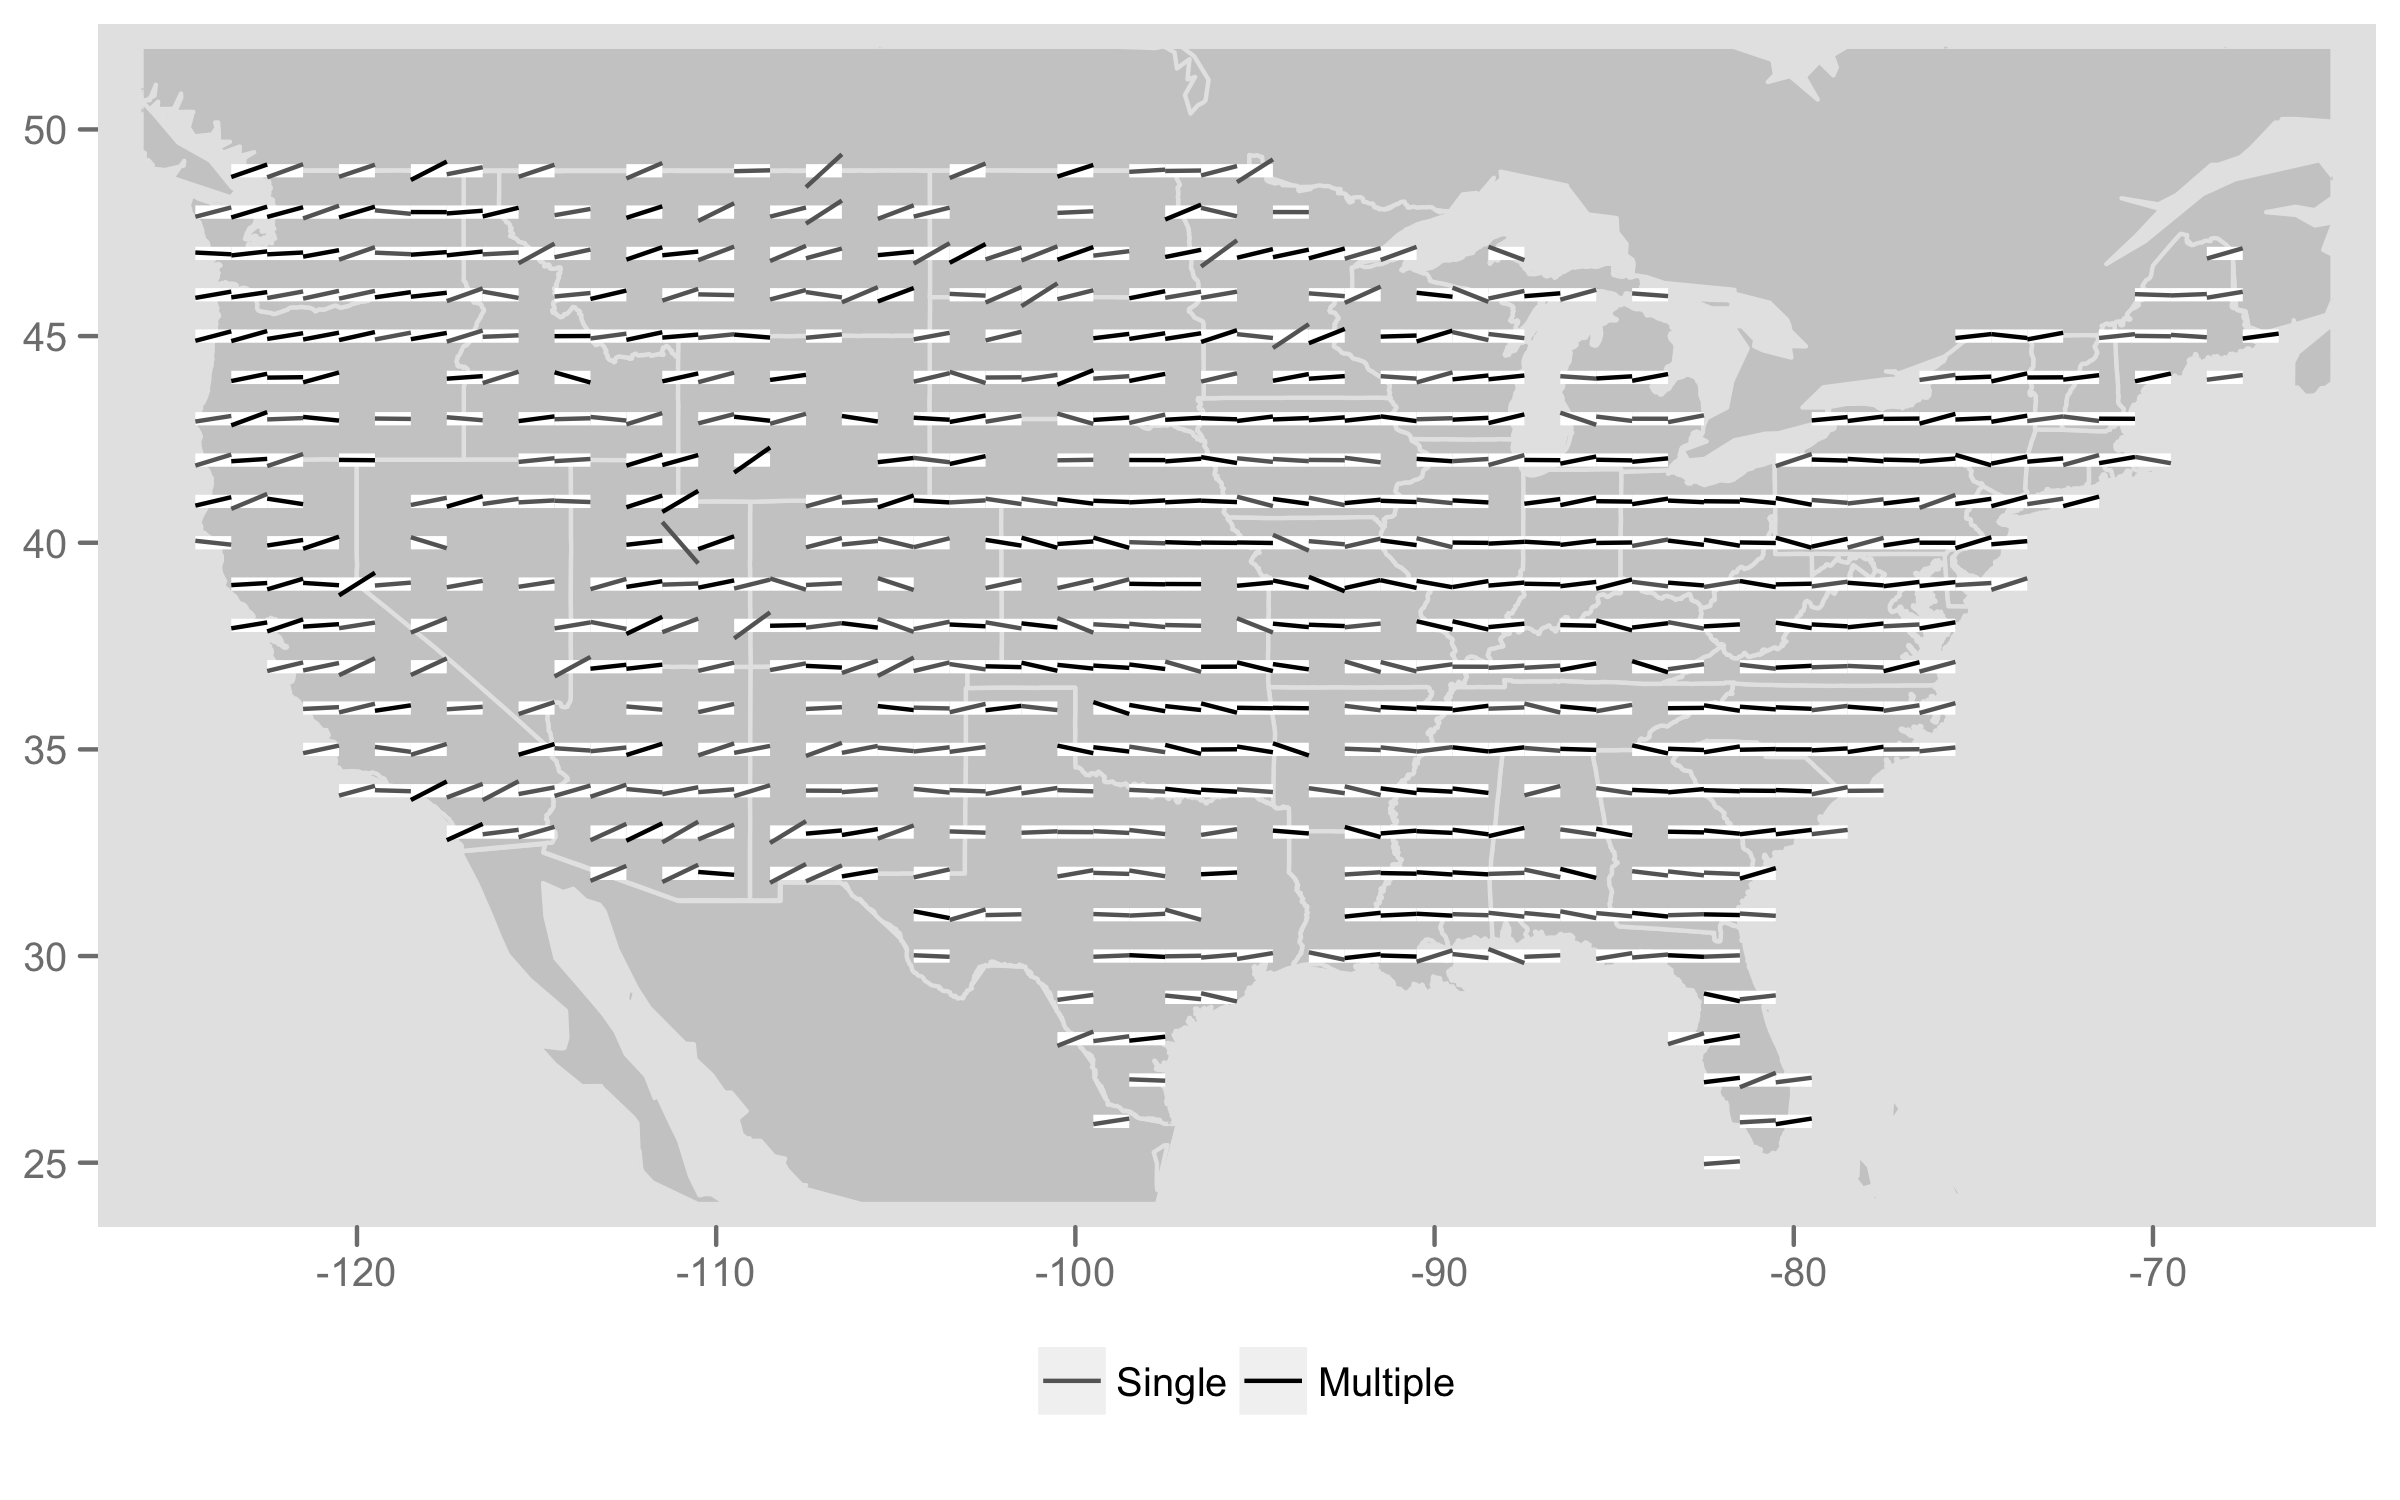
\includegraphics[width=0.5\linewidth]{usa-lin-grid}%

  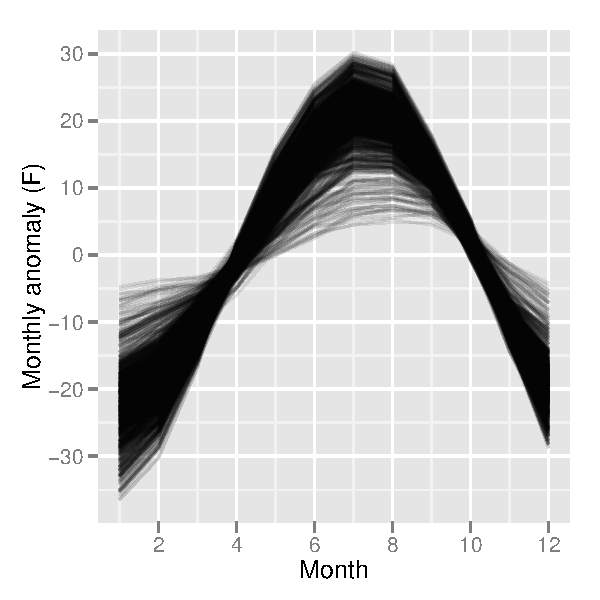
\includegraphics[width=0.20\linewidth]{usa-season-legend}\hspace{2in}%
  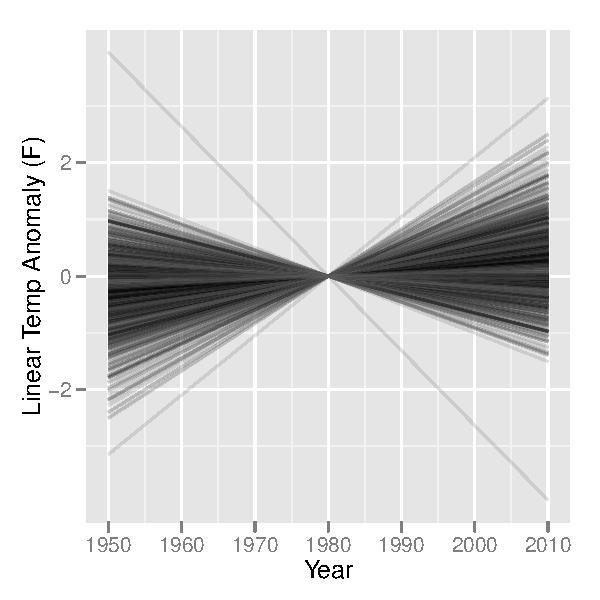
\includegraphics[width=0.20\linewidth]{usa-lin-grid-legend}
  \caption{Glyph-maps of seasonal patterns (top left) and linear trends (top right) of USHCN stations, 1950--2010.  Station locations have been rounded to the nearest degree Each location has a glyph in the seasonal plot and color of the tiles corresponds to the average temperature of the locations. Heavy lines in the linear trend plot correspond to average trends over more than one location. (Bottom) Legends showing scale of glyphs.} 
  \label{fig:irregular-grid}
\end{figure}

Reference guides become especially important in the irregularly gridded data. Comparisons are harder because comparing icons along a common baseline, be it along a row or column of glyphs, is absent. Without reference lines or boxes it is also hard to compare line lengths, to tell if short series are missing data at the start or end. In each of the plots in Figures \ref{fig:irregular}, \ref{fig:irregular-collapsed} and \ref{fig:irregular-grid}, reference lines or boxes have been included. 

\begin{figure}[htbp]
  \centering
  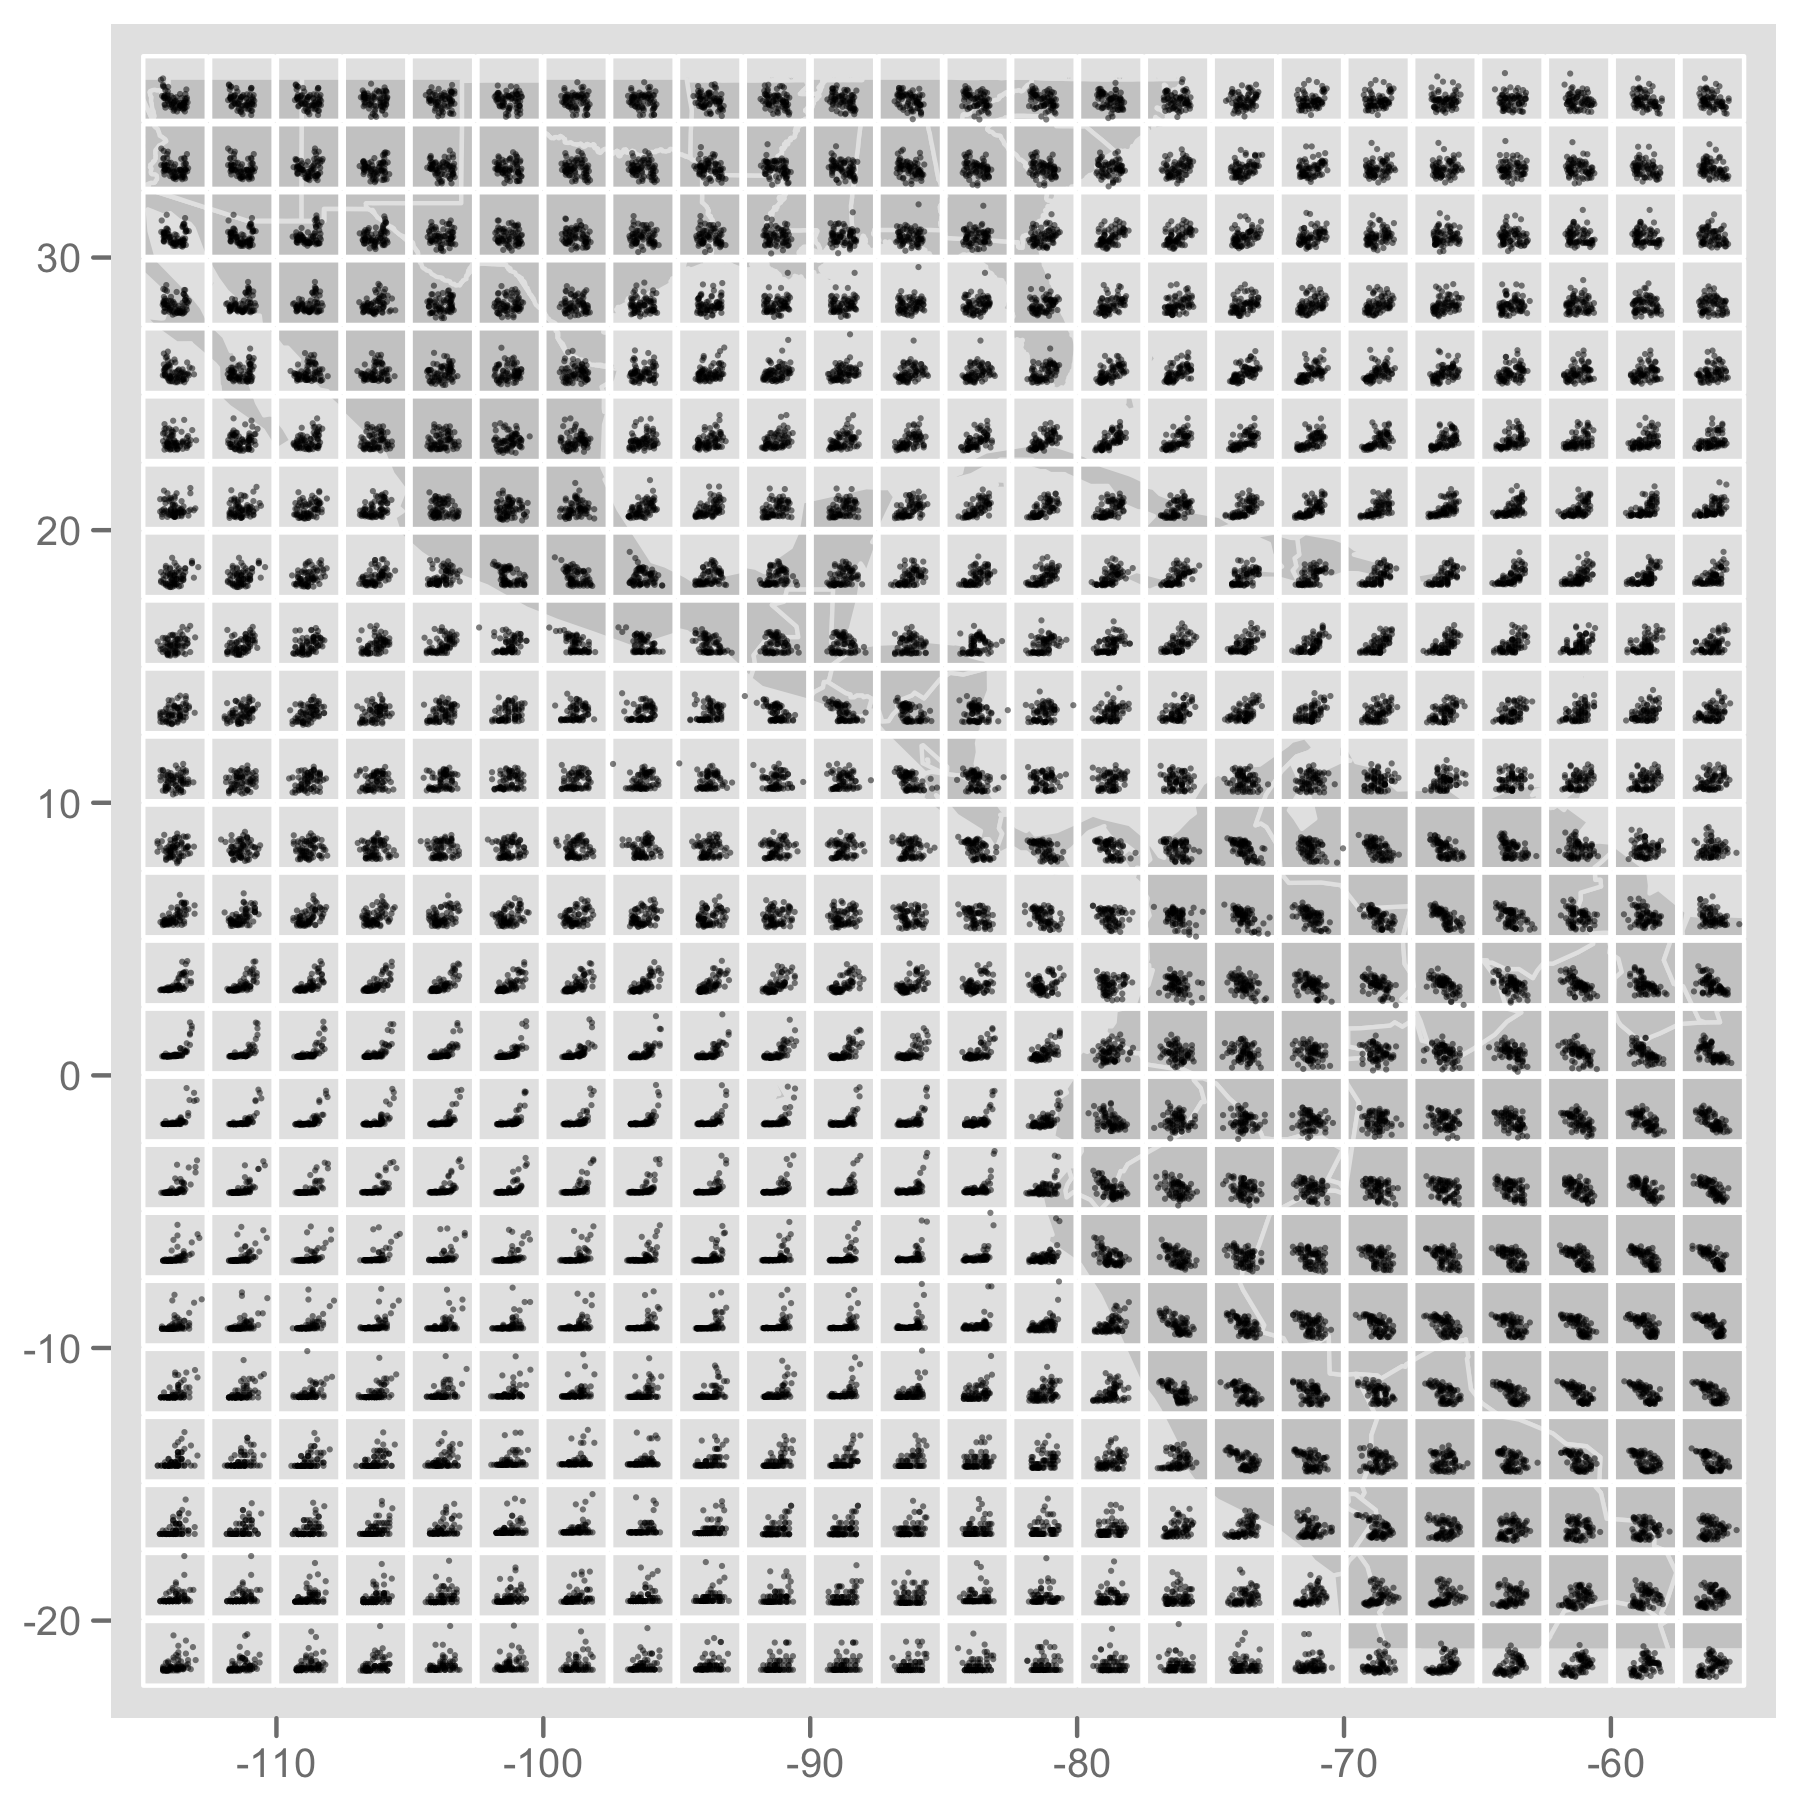
\includegraphics[width=0.5\linewidth]{nasa-scat-glyph}%
  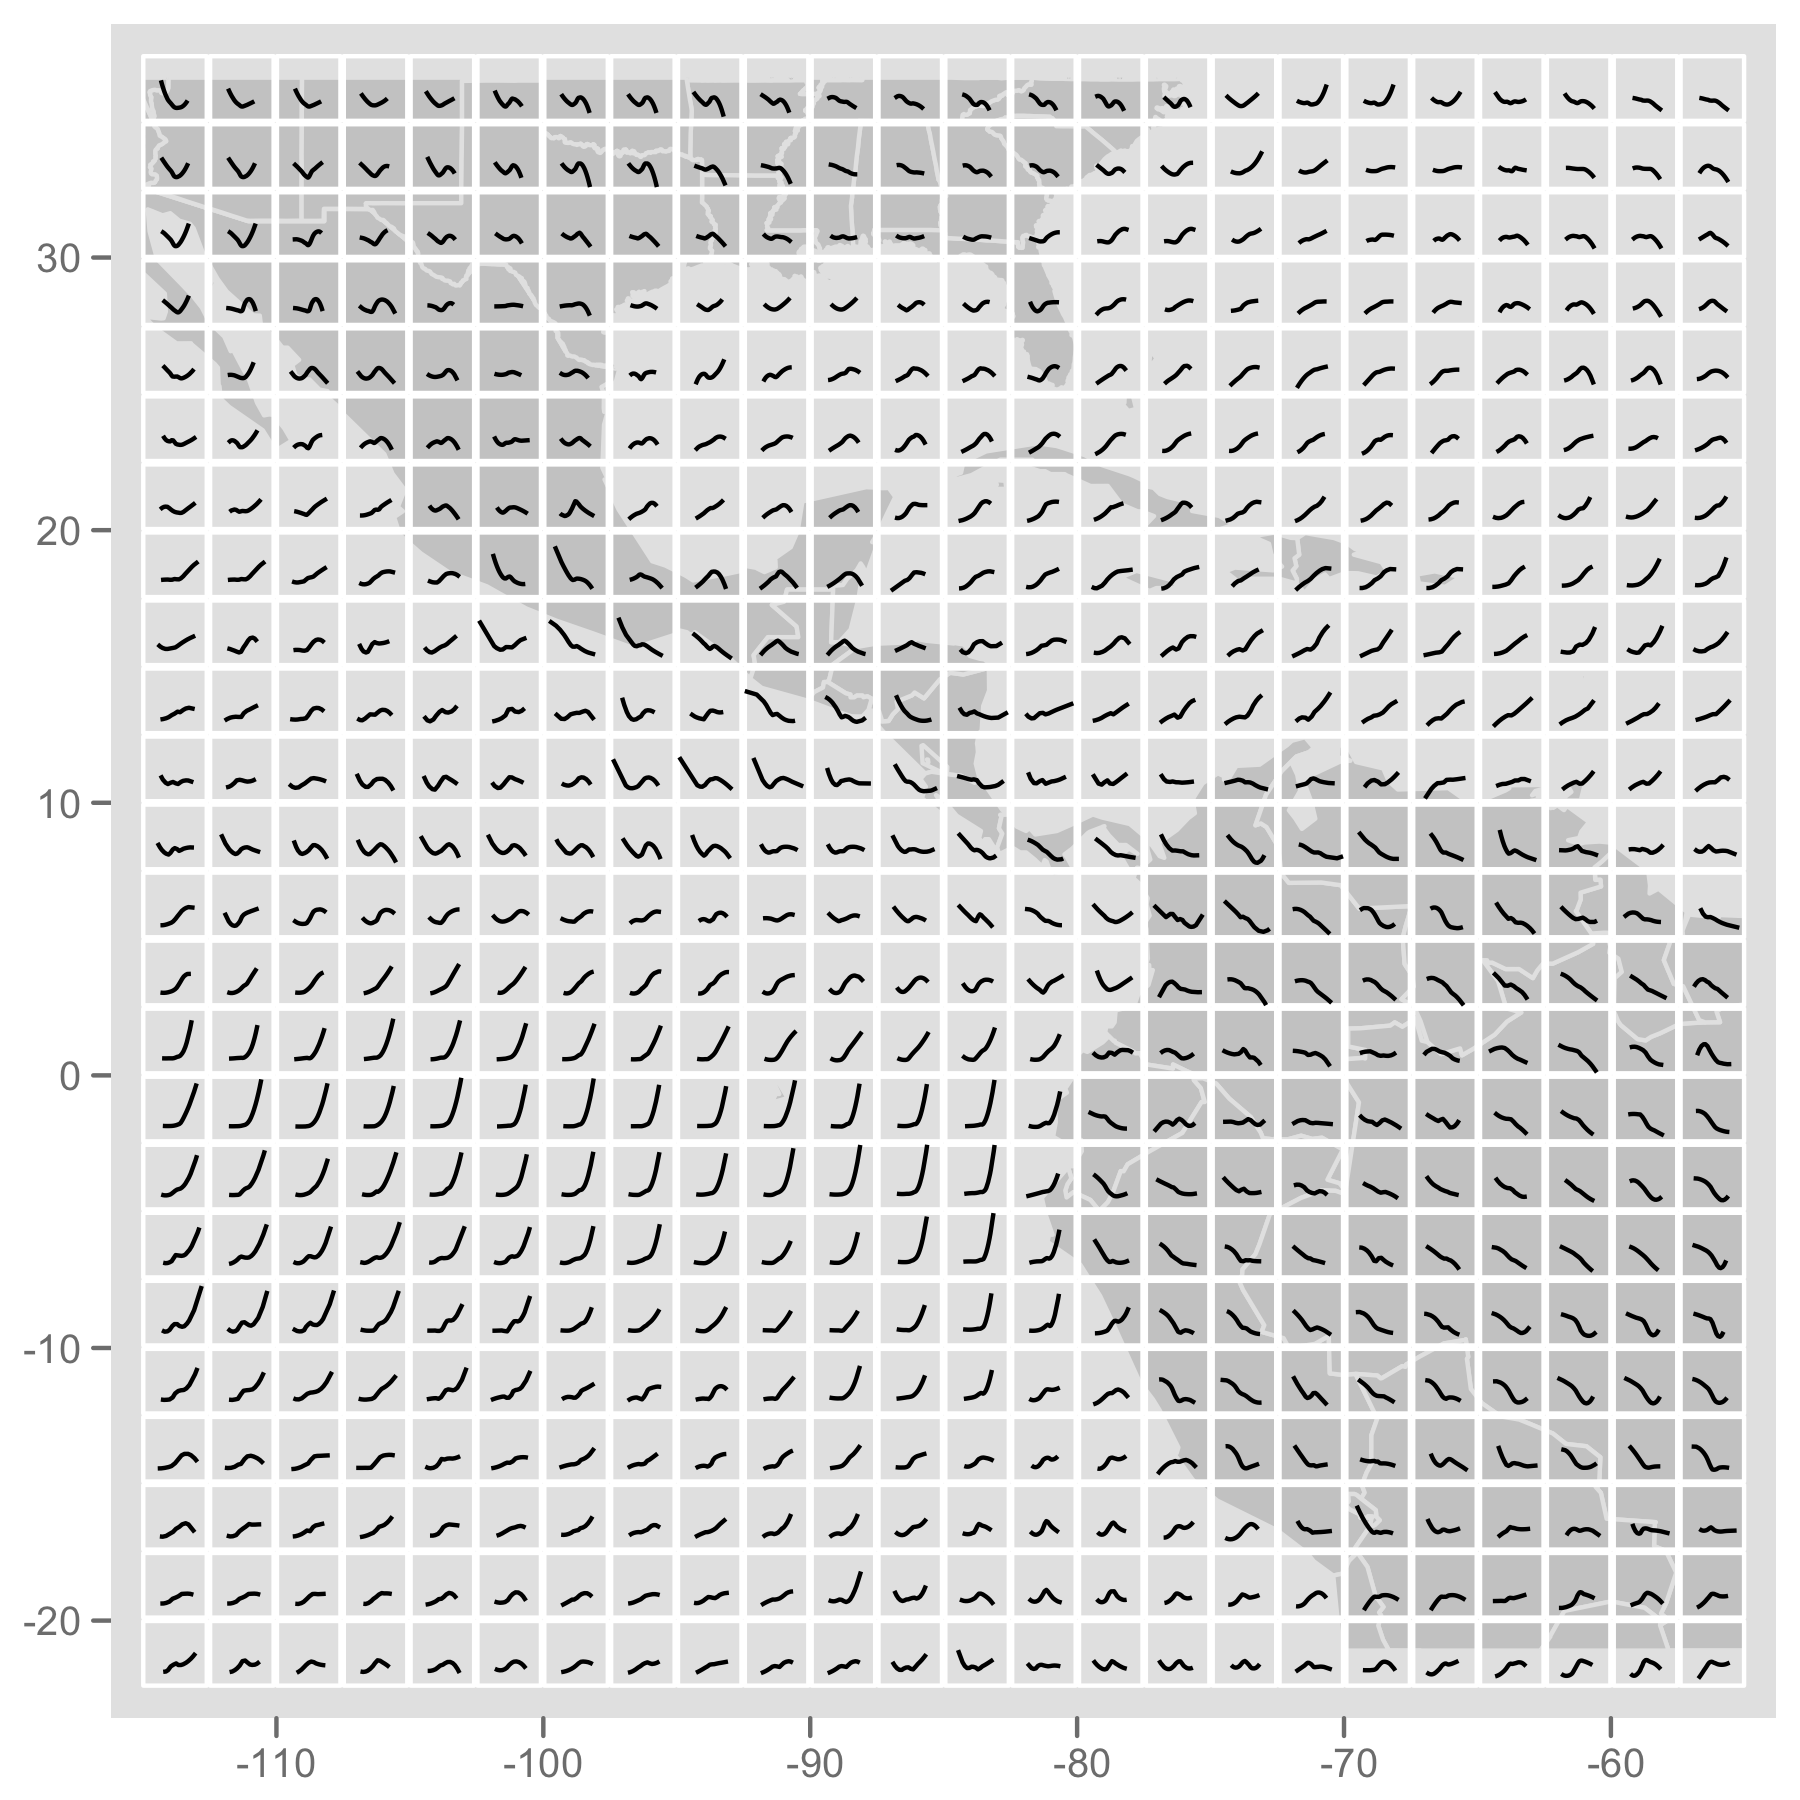
\includegraphics[width=0.5\linewidth]{nasa-loess-glyph}

  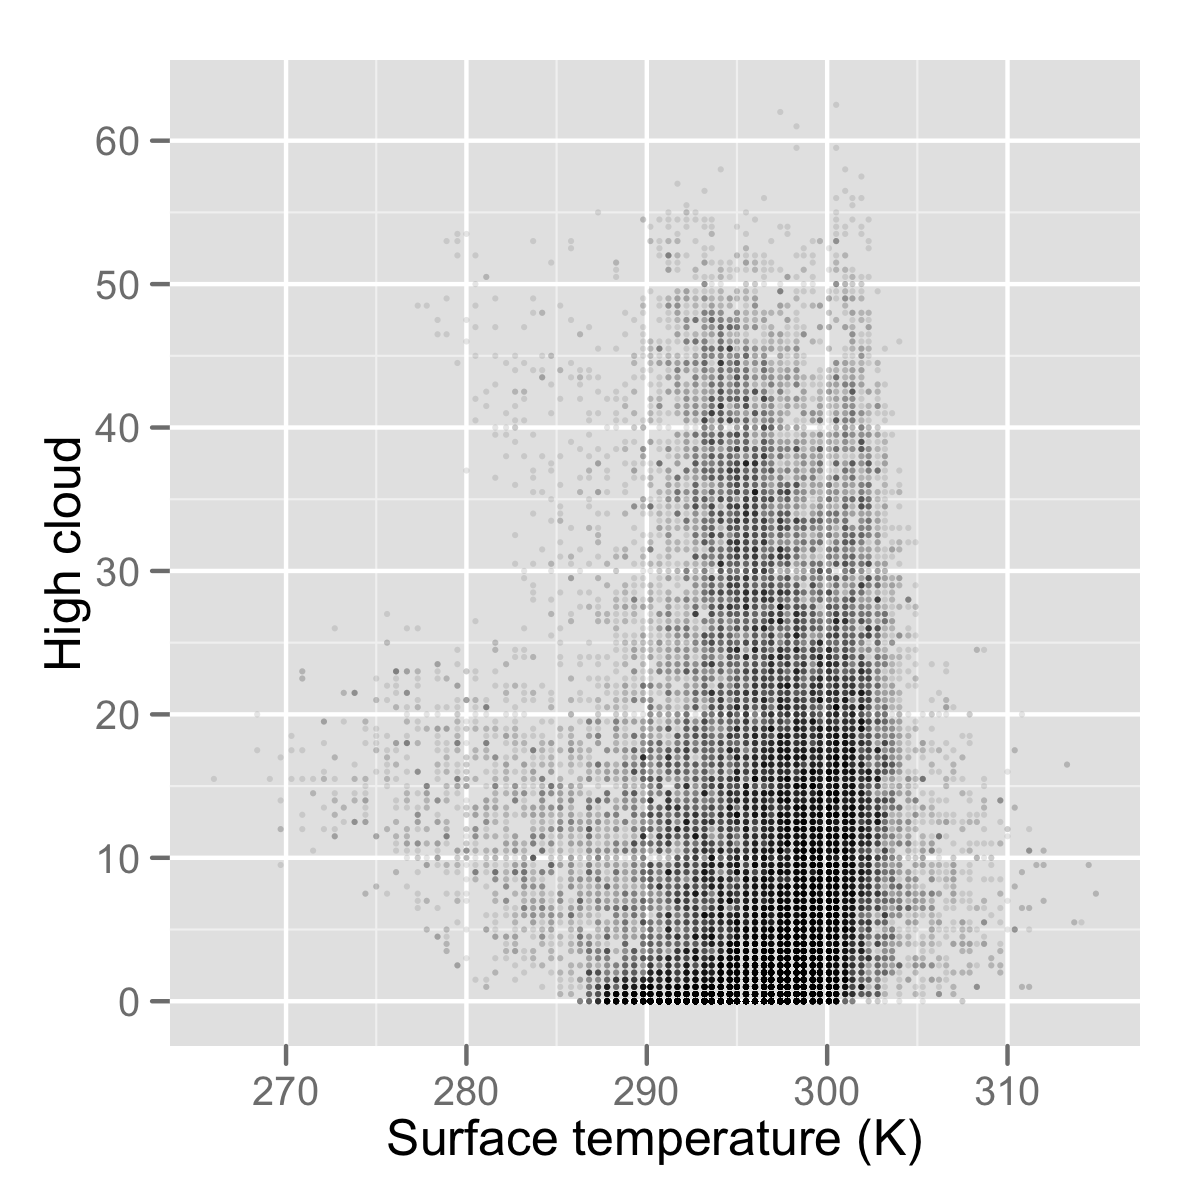
\includegraphics[width=0.20\linewidth]{nasa-scat-legend}%
  \hspace{0.17\linewidth}%
  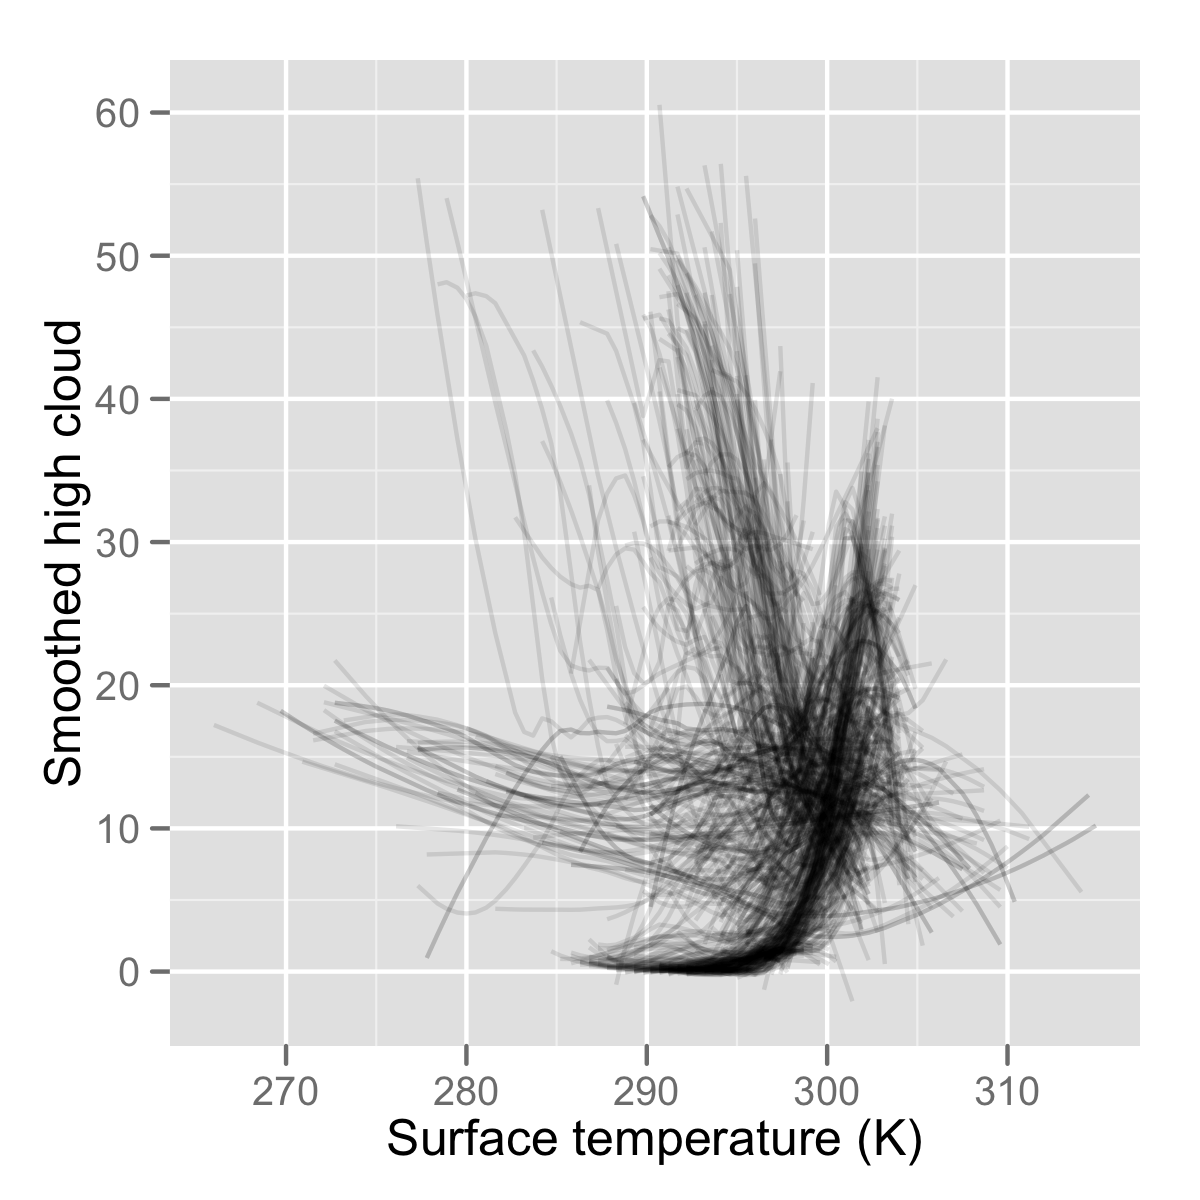
\includegraphics[width=0.20\linewidth]{nasa-loess-legend}

  \caption{Glyph-map showing (top left) scatterplot of temperature vs high-cloud and (top right) smoothed (loess) curve fit to each location. The relationship between these two variables varies considerably over the spatial domain. (Bottom) Legends show overall patterns and scales.}
  \label{fig:cloud}
\end{figure}

\section{Generalizations}

Glyphs, of course, can be more general than lines or stars. For multivariate data we may want to represent several variables ($z_1, \dots, z_p; p=$ number of variables) in the glyphs. Figure~\ref{fig:cloud} shows scatterplots of the EXPO data as icons: temperature values ($z_1$ instead of $t$) are displayed horizontally and high-cloud values ($z_2$) are displayed vertically, both locally scaled. The bivariate relationship between the two variables is explored spatially: the equatorial Pacific and Caribbean have positive association between temperature and high cloud, while the south American continent has negative association. The right side plot displays a loess curve fit to the data instead of the individual points, sharpening the association signal relative to the variation. Gauguin \citep{gribov:2006}, has an icon based on a histogram, giving small univariate distribution displays for each location. \citet{carr:1992} use ray glyphs to show bivariate relationships.

\section{Discussion}

There are two natural next directions for this work: perceptual experiments, and development of interactive graphics. Several careful studies comparing the perceptual elements of these displays, using different scale and glyph options, and in comparison with facetted heatmaps, would be recommended. For example, it appears that periodic trends are easier to perceive in star-glyphs, and long-term trends in line-glyphs. Is this always the case? Are there certain types of periodicity that are particularly easy to spot? Rigorous perceptual studies will help guide the use of glyph-maps.

The conceptualization and equations for computing the glyph-maps lend themselves to producing these displays interactively. Different variables can be swept into the display using mouse motion mapped to $\alpha_x, \alpha_y$ (Equation \ref{coords.eqn}), resolution could be increased, and aggregated data icons disengaged, upon zooming into a spatial neighborhood. This experimentation is ideally done using R, so that computation can be linked with displays. The hurdle has been the lagging development of interactive graphics in R. Several new packages  in R have become available in the past year \citep{qtbase, qtpaint, plumbr} that support interactive graphics which will enable these developments.

In summary, glyph-maps enable the study of temporal patterns in multivariate spatiotemporal data. Climate change is focused on changes over time, so glyph-maps provide a way to explore these changes directly. Glyph-maps enable different resolutions of the data to be examined: the raw data to discover data quality issues, global trend, seasonality, residuals, and multivariate dependencies. When the data is spatially gridded the glyphs are organized in a manner that makes reasonable comparisons. For irregularly gridded data the icon size needs to be chosen to minimize overlap but use as much display space as possible, or combined to produce close to gridded icons. 

\section*{Acknowledgements}

This work was partially supported National Science Research grant DMS0706949.

\bibliography{references}

\end{document}